% LaTeX Vorlage für studentische Arbeiten am imes, MZH, ...
% Vorlagenversion vom 15.08.2017
%
%
%
%
%
% META & VOREINSTELLUNGEN -------------------------------------------------------
\newcommand{\Autor}%                % Name des Autors / der Autorin
{Adrian Kleimeier}
\newcommand{\Matrikelnummer}%       % Matrikelnummer
{3111950}
\newcommand{\Datum}%       % Abgabedatum
{15. Januar 2021}

% ------------------------------------------------------------------------------------------
% erlaubt das Anfangen des Draft-Modus und damit Veränderungen
% einzustellen
\newif\ifdraft
% Draft-Modus: Arbeitsversion, Bilder werden nur als Rahmen dargestellt
% Vorteil: schnelleres Kompilieren
%\drafttrue % <- dafür hier die Kommentierung wegnehmen

%-------------------------------------------------------------------------------------------
% folgende Befehle sorgen dafür, das für jede Schrift die richtigen Pakete installiert werden
\newcounter{schrift}
% Schrift auswählen:
% 1 - mathptmx
% 2 - minionpro
% 3 - mathpazo
% 4 - times + computer modern
% 5 - computer modern
\setcounter{schrift}{4} % Hier die entsprechende Zahl setzen !

% ------------------------------------------------------------------------------------------
% ------------------------------------------------------------------------------------------
% Latex - Präambel
% hier werden alle wichtigen Dokumenteinstellungen getroffen, normalerweise müssen
% keine Änderungen mehr durchgeführt werden.
% Pakete die das Schriftbild, den Satzspiegel oder die Ränder verändern, dürfen
% nicht hinzugefügt werden, erst nach Abstimmung mit dem Betreuer.
% nützliche Pakete sind willkommen, bitte die Wiki entsprechend aktualisieren
% viele Pakete sind drin, die vielleicht nicht jeder braucht und das Kompilieren verlängern
% sollten diese das Layout nicht verändern, können diese natürlich auskommentiert werden.
% ------------------------------------------------------------------------------------------

% ------------------------------------------------------------------------------------------
% Dokumentenklasse definieren:
\ifdraft
    \documentclass[draft, 
                   paper=a4,
                   BCOR=5mm,
                   fontsize=12pt, 
                   headsepline, 
                   numbers=noenddot, 
                   %bibtotoc,
                   bibliography = totoc,
                   %version=first,
                   %smallheadings,
                   headings = small,
                   oneside]{scrbook}
\else
    \documentclass[paper=
                   a4,
                   BCOR=5mm,
                   fontsize=12pt, 
                   headsepline, 
                   numbers=noenddot, 
                   %bibtotoc,
                   bibliography = totoc, 
                   %version=first,
                   %smallheadings,
                   headings = small,
                   headinclude=true,
                   footinclude=false,
                   %fleqn, % formeln links bündig
                   oneside]{scrbook}
\fi
% Standard-Koma-Dokument mit
%   Papierformat A4
%   Binderand 5 mm
%   Schrift 12-Punkt
%   Seitenlayout nach DIV, siehe scrguide.pdf text b/h rand oben/innen: 168,00 237,60 19,80 14,00 (ist raus)
%   Linie unter der Kopfzeile
%   Nummern ohne Punkt am Ende
%   Literaturverzeichnis im Inhaltsverzeichnis
%   Überschriften etwas kleiner als standard
%   weitere Informationen zum Koma-Skript: www.komascript.de

%---------------------------------------------------------------
% Basis-Pakete
%---------------------------------------------------------------
\usepackage{ifpdf}		%   Ueberprueft, ob LaTeX oder pdfLaTeX verwendet wird (nur ab MikTeX 2.5)
\usepackage[T1]{fontenc}        %   8-Bit-Fonts
\usepackage{textcomp,latexsym}  %   zusaetzliche Symbole
\usepackage[utf8]{inputenc}   %   Quelltext ist Latin-1 (d.h. Windows-) kodiert
\usepackage{csquotes}
\usepackage[ngerman]{babel}            %   neue deutsche Rechtschreibung
\usepackage[
    style=alphabetic,
    maxbibnames=99
]{biblatex}
\usepackage{scrtime}            %   fuer die aktuelle Zeit
%\usepackage{scrdate}            %   fuer das aktuelle Datum
%\usepackage{natbib}             %   Literaturverweise mit (Autor Jahr) nach DIN
%\bibpunct[; ]{[}{]}{,}{a}{}{;}  %   eckige Klammern statt runde bei Zitaten
%\usepackage[T1]{url}            %   Web-Addressen auch mit T1-Encoding
%\urlstyle{tt}                   %   und in tt-Font
%\usepackage[activate=normal]{pdfcprot} % dient dem optischen Randausgleich bei kürzeren Zeichen wie '-', '.', ',', '!'

\usepackage{color}

\PassOptionsToPackage{x11names}{xcolor}
\usepackage{xcolor}
\usepackage{booktabs}

%---------------------------------------------------------------
% nützliche Zusatz-Pakete
%---------------------------------------------------------------
%\usepackage{makeidx}            %   Index (wenn gewuenscht)

\usepackage{setspace}           %   Zeilenabstand setzen. Befehl:
                                %   \begin{spacing{Wert}
                                %   Text
                                %   \end{spacing}
%\usepackage{placeins}           %   das Positionieren von float-Umgebungen bestimmen:
                                %   der Befehl \floatbarrier sorgt dafür, dass alle vorher eingegebenen
                                %   float-Umgebungen VOR diesem Befehl eingefügt werden.
                                
%\usepackage{subfig}          %   Bilder gruppieren, mehrere Bilder in einer Umgebung einfügen
                                %   Bsp.:
                                %   \begin{figure}
                                %   \centering
                                %    \subfloat[Text a]
                                %    {\includegraphics{bild a}}
                                %    \subfloat[text b]
                                %    {\includegraphics{bild b}}
                                %    \caption{Untertitel}
                                %    \label{fig.Beziechnung_subfigure} <- am besten mit fig. dann kann mit \bild{Bezeichnung_figure} referenziert werden
                                %   \end{figure}                                

%\usepackage{textcomp}           %   fuer Trademark und Copyright Zeichen
                                %   z.B \texttrademark, \textregistered, \texteuro etc.

\usepackage{tabularx}           %   erweiterte Funktionen für Tabellen

\usepackage{longtable}          %   Longtable-Package für Tabellen die länger als eine DIN-A4-Seite sind

\usepackage{colortbl}						%		farbige Tabellenzeilen

\usepackage{nicefrac}           %   Schräge Bruchstriche \nicefrac{Nenner}{Zähler}

%\usepackage{numprint}           %   Zahlen mit Einheiten näher an der Zahl/kein Umbruch und 1 000er Format \numprint[Einheit]{Zahl}

%\usepackage{mathcomp}           %   für \tcdegree (° Gradzeichen bei numprint) \numprint[\tcdegree]{180} für 180°

%\usepackage{hhline}             %   hhline-Package
                                %   Fuer komplexe Linienzuege in Tabellen \hhline{}
                                %   = Spalte mit doppelter Linie      | vertikale Linie die horizontale schneidet
                                %   - Spalte mit einfacher Linie      : vertikale Linie die von horizantaler unterbrochen ist
                                %   ~ Spalte ohne Linie               # doppelte horiz. geschnitten mit doppelter vert. Linie
                                %   t oberer Teil ->                  b unterer Teil einer doppelten Linie

%\usepackage[active]{srcltx}     %   bei verwendung v. \includeonly spring winedt jetzt bei fehlern an die richtige stelle

\usepackage{flafter}            %   Ein float-Objekt immer erst NACH seiner Definition platzieren

\usepackage{ifthen}             %   definiert \ifthenelse{}{}{}

%\usepackage{path}               %   dateinamen und pfade darstellen

%\usepackage{pdfsync}						%   Synchronisation mit SumatraPDF <<-- geht auch ohne

\usepackage{booktabs}

%% Eigene Pakete

\usepackage{scrhack} % Löscht Warnungen von Packages wie hyperref, listings
\usepackage[ locale = DE,            % deutsch
            load-configurations=abbreviations, % zusätzliche Einheiten siehe manual
            per-mode=symbol,%-or-fraction,
            separate-uncertainty% 
            ]
            {siunitx}								% SI-Einheiten  
						\sisetup{detect-all} % aktuelle Schriftart nutzen (statt immer Mathemodus)

            
\usepackage{multirow}               % zwei Zeilen kombinieren (wie multicolumn)
\usepackage[babel]{microtype}       % schickeres Schriftbild -> aber längeres Kompilieren

\usepackage{blindtext}							% sinnlosen text einbauen
\usepackage{subfigure}

\usepackage{newunicodechar}
%\newunicodechar{ }{~}

%\DeclareUnicodeCharacter{00A0}{~}


%%

%---------------------------------------------------------------
% Grafik-Paket für eps bzw. pdf
%---------------------------------------------------------------
% überprüft ob Latex oder PDFLatex ausgeführt wird, dementsprechend werden pdf/jpg oder eps Bilder eingefügt
% sollen dvi oder pdf Dokumente erstellt werden müssen alle Bilder in beiden Formaten vorliegen
% hierfür gibt es Tools wie epstopdf oder jpgtoeps
 \ifdraft
    \usepackage[draft]{graphicx}
\else
    \ifpdf
        \usepackage{graphicx}
        \usepackage{pgfplots} % pgfplots zum plotten in LaTeX
    \else
        \usepackage[final]{graphicx}
    \fi
\fi
% von wo sollen die Grafiken kommen?
\graphicspath{{./Abbildungen/}}

%Einstellungen für pgfplots
\pgfplotsset{compat=1.3,
	%enlargelimits=auto,
	tick label style={font=\small,/pgf/number format/use comma}, %Komma nutzen in allen Axen
	%axis x line=center, %alle x-Achsen center
	%axis y line=center, %alle y-achsen center
	%every axis x label/.style={at={(current axis.right of origin)},anchor=west}, % achsenbeschriftung bei allen x-achsen rechts
	%every axis y label/.style={at={(current axis.above origin)},anchor=south},   % achsenbeschriftung bei allen y-achsen oben
	%every x tick scale label/.style={at={(current axis.right of origin)},anchor=north,yshift=-0.5em}, %positionierung des scale faktors geändert
	every axis legend/.append style={at={(0.5,1.03)},anchor=south,nodes=right,font=\small}, % Legende über der Grafik, schriftgröße small
	label style={font=\small} % label schriftgröße small
}
\newlength\tikzwidth
\setlength{\tikzwidth}{0.7\textwidth}
\definecolor{mycolor1}{rgb}{0,0.5,0}

\ifpdf
 \ifdraft
    \usepackage[draft]{pdfpages}%   externe PDF Seiten einbinden nur bei PDF-Latex möglich
    \else
    \usepackage[final]{pdfpages}%   externe PDF Seiten einbinden nur bei PDF-Latex möglich
 \fi                            %   Befehl: \includepdf{PDF-Datei} soll die Datei im Querformat angezeigt werden
    \else
\fi                             %   \includepdf[landscape=true]{PDF-Datei}

%---------------------------------------------------------------
% Debug-Ausgabe der Labels und References
%---------------------------------------------------------------
\ifdraft
  \usepackage{showkeys} % Label werden im Draft Modus im Text angezeigt
\fi

%---------------------------------------------------------------
% Abweichende PostScript-Schriftarten
% werden in der main Datei ausgewählt, hier nichts ändern
%---------------------------------------------------------------
\ifthenelse{\equal{ 1 }{ \value{schrift} }}
    {
    \usepackage{mathptmx}          %   Times als Hauptschriftart, keine mathematische Fettschrift
    \usepackage{amssymb}
    \usepackage{amsbsy}
    \usepackage{amsmath}
    \usepackage{amsfonts}
    \usepackage{amstext}
    \renewcommand{\boldsymbol}[1]{\mathbf{#1}} % nur bei mathptmx !
                                               % damit boldsymbol wenigstens fette aufrechte Buchstaben macht
    }{}
\ifthenelse{\equal{ 2 }{ \value{schrift} }}
    {
    \usepackage[lf, minionint]{MinionPro} %   OpenType von Adobe, mathematische Fettschrift vorhanden, Schrift ist
                                %   ist im Standard-LaTeX nicht installiert.
                                %   Ist ein wenig Aufwand das Ganze zu installieren, Matthias Dagen fragen
    }{}
\ifthenelse{\equal{ 3 }{ \value{schrift} }}
    {
    \usepackage{mathpazo}          %   nette Buchschrift aber sehr gross, mathematische Fettschrift vorhanden
    \usepackage{amssymb}
    \usepackage{amsbsy}
    \usepackage{amsmath}
    \usepackage{amsfonts}
    \usepackage{amstext}
    }{}
\ifthenelse{\equal{ 4 }{ \value{schrift} }}
    {
    \usepackage{times}
    \usepackage{amssymb}
    \usepackage{amsbsy}
    \usepackage{amsmath}
    \usepackage{amsfonts}
    \usepackage{amstext}
    }{}
\ifthenelse{\equal{ 5 }{ \value{schrift} }}
    {
    \usepackage{amssymb}
    \usepackage{amsbsy}
    \usepackage{amsmath}
    \usepackage{amsfonts}
    \usepackage{amstext}
    \usepackage{lmodern}
    }{}
\usepackage[scaled=.92]{helvet} %   11pt Helvetica für Überschriften etc. etwas kleiner da, Helvetica an sich größer ist
%\usepackage{courier}            %   Courier bei \texttt
%\usepackage{upgreek}            %   Aufrechte griechische Buchstaben

% ------------------------------------------------------------------------------------------
% Bild- und Tabellentitel FETT
% ------------------------------------------------------------------------------------------
%\def\figurename{\bfseries Bild}
%\def\tablename{\bfseries Tabelle}

%%Andere Beschreibung von figure
\addto\captionsngerman{
	\renewcommand{\figurename}{\bfseries Bild}%%Andere Beschreibung von figure
	\renewcommand{\listfigurename}{Bildverzeichnis}
	\renewcommand{\tablename}{\bfseries Tabelle}
}

%---------------------------------------------------------------
% Quelltexte formatieren
%---------------------------------------------------------------
\usepackage{listings}


%\lstloadlanguages{
		%C,
		%C++,
		%XML
%}

\lstset{
		language=XML,
		basicstyle=\footnotesize\ttfamily, % Standardschrift
		numbers=left,               % Ort der Zeilennummern
		numberstyle=\tiny,          % Stil der Zeilennummern
		numbersep=5pt,              % Abstand der Nummern zum Text
		tabsize=2,                  % Groesse von Tabs
		extendedchars=true,         %
		breaklines=true,            % Zeilen werden Umgebrochen        
		keywordstyle=\color{Red2},
		frame= b,         
		stringstyle=\color{Purple2}\ttfamily, % Farbe der String
		showspaces=false,           % Leerzeichen anzeigen ?
		showtabs=false,             % Tabs anzeigen ?
		xleftmargin=17.5pt,
		framexleftmargin=17pt,
		framexrightmargin=5pt,
		framexbottommargin=4pt,
		linewidth= \dimexpr\textwidth-2\fboxsep-2\fboxrule,
		comment=[l]{\#},
		morecomment=[s]{<!--}{-->},
		commentstyle=\color{Green4},
		%backgroundcolor=\color{grey},
		showstringspaces=false,      % Leerzeichen in Strings anzeigen ?        
		morekeywords={__global__, name, pkg, args, type, from, to, textfile, respawn, value, output, radius, ixx, ixy, ixz, iyy, iyz, xyz, rpy, reference},  % CUDA specific keywords
		aboveskip = 18pt, 
		belowskip = 18pt
}

\usepackage{caption}
\DeclareCaptionFont{white}{\color{white}}
\DeclareCaptionFormat{listing}{\colorbox{darkgray}{\parbox{\dimexpr\textwidth-2\fboxsep-2\fboxrule}{\hspace{15pt}#1#2#3}}}
\captionsetup[lstlisting]{format=listing,labelfont=white,textfont=white, singlelinecheck=false, margin=0pt, font={bf,footnotesize}}

%---------------------------------------------------------------
% ein paar Längen einstellen
%---------------------------------------------------------------
%\setlength{\parskip}{1ex plus0.5ex minus0.2ex} % Absatzabstand etwas größer
\setlength{\itemsep}{0ex plus0.2ex}            % Abstand zweier Listenelemente kleiner
\setlength{\parindent}{0ex}                     % kein Absatzeinzug
\setlength{\belowcaptionskip}{0.4cm}            % Abstand caption - Tabelle größer
\setlength{\abovecaptionskip}{0.4cm}            % Abstand caption - Tabelle größer

%---------------------------------------------------------------
% Kopf- und Fusszeilen
%---------------------------------------------------------------
\usepackage[plainheadsepline,  % linie zw. kopf und text auch bei seitenstil "plain"
           %headexclude,       % kopfzeile gehört nicht zum textkörper
           %footexclude        % fusszeile gehört nicht zum textkörper
          ]       
           {scrlayer-scrpage}
\pagestyle{scrheadings}
\clearpairofpagestyles              % voreinstellungen loeschen
\ihead{\normalfont\headmark}   % kolumnentitel innen
\ohead[\pagemark]{\pagemark}   % seitenzahl aussen

%---------------------------------------------------------------
% Nummerierungs-Tiefe des Inhaltsverzeichnis und der Abschnitte einstellen
%---------------------------------------------------------------
\setcounter{secnumdepth}{2} \setcounter{tocdepth}{2}

%---------------------------------------------------------------
% Abkürzungsverzeichnis
%---------------------------------------------------------------
% mit dem Befehl \nomenclature[l/g/a]{Abkürzung}{Bezeichnung} kann direkt im Code die Abkürzung eingefügt werden
% das Paket sortiert diese und fügt sie mit dem Befehl \printnomenclature ein
% l, g, oder a steht dabei für die Gruppierung Lateinische bzw. Griechische Buchstaben, Abkürzungen
% Nach Einfügen neuer Abkürzungen muss folgender Befehl in der Eingabeaufforderung im Tex-Verzeichnis eingegeben werden:
% -> vorher einmal kompilieren
% -> makeindex main.nlo -s nomencl.ist -o main.nls
% -> nochmal kompilieren
%\makeindex
\usepackage{nomencl}
% \let\abbrev\nomenclature
\renewcommand{\nomname}{Abkürzungsverzeichnis}
\setlength{\nomlabelwidth}{.25\hsize}
\renewcommand{\nomlabel}[1]{#1 \hfill}
\setlength{\nomitemsep}{-\parsep}

\renewcommand{\nomgroup}[1]{%
	\ifthenelse{\equal{#1}{L}}{\item[\textbf{Lateinische Buchstaben}]}
	{%
		\ifthenelse{\equal{#1}{G}}{\item[\textbf{Griechische Buchstaben}]}
		{%
			\ifthenelse{\equal{#1}{A}}{\item[\textbf{Abkürzungen}]}
			{
				\ifthenelse{\equal{#1}{K}}{\item[\textbf{Koordinatensysteme}]}{}
			}
		}
	}
}

\makenomenclature

%---------------------------------------------------------------
% Hyperlinks für pdfTeX
%---------------------------------------------------------------
\ifpdf
    % hier stehen befehle, die nur für pdftex gelten
    \usepackage[pdfpagelabels,  % logische (z.b. auch roemische) seitenzahlen
                bookmarks,       % Bookmarks für die einzelnen Abschnitte
                pdftex
                ]{hyperref}
    \hypersetup{
    %   colorlinks,  % Links mit farbigem Text
        pdfborder   = 0 0 0,
        plainpages  = false,
        bookmarksnumbered = true,
    %   bookmarksopen
    }
\else
    % hier stehen befehle, die nur für latex gelten
    \usepackage{hyperref} % hier ohne colorlinks und pdf-krams
\fi

%---------------------------------------------------------------
% SVGs einfügen
%---------------------------------------------------------------
%% SVG to TeX
% from InkscapePDFLaTeX.pdf
% by Johan Engelen, 2010
% Information: 
% http://tug.ctan.org/tex-archive/info/svg-inkscape
% -shell-escape muss im Ausgabeprofil stehen
% inkscape.exe muss im Path-Folder sein

% Funktion zum ueberpruefen auf Aenderung
\newcommand{\executeiffilenewer}[3]{%
                \ifnum\pdfstrcmp{\pdffilemoddate{#1}}%
                {\pdffilemoddate{#2}}>0%
                {\immediate\write18{#3}}\fi%
}
% Wenn Aenderung dann TeX-Export ausfuehren und einbinden
%\newcommand{\includesvg}[1]{%
                %\executeiffilenewer{#1.svg}{#1.pdf}%
                %{inkscape -z -C --file=#1.svg %
                %--export-pdf=#1.pdf --export-latex}%
                %\input{#1.pdf_tex}%
%}

%% Include svg mit Text aus textext plugin
% text wird im svg mit textext hinzugefügt.
% falls Änderungen im .svg gefunden werden, wird das Bild 
% neu exportiert und eingefügt.
% \includesvg{ordner/file} /ohne endung
\newcommand{\includesvg}[4][]{
			\executeiffilenewer{#3.svg}{#3.pdf}
			{inkscape -z -D --file=#3.svg
			--export-pdf=#3.pdf}
			\begin{figure}[#2]
				\centering
				\includegraphics[#1]{#3}
				\caption{#4} \label{fig.#3}
				\vspace*{-3mm}
			\end{figure}
}

\newcommand{\includesinglesvg}[2][]{
			\executeiffilenewer{#2.svg}{#2.pdf}
			{inkscape -z -D --file=#2.svg
			--export-pdf=#2.pdf}
			\includegraphics[#1]{#2}
}

\usepackage[right]{eurosym}

                  % Präambel zur Dokumentenformatierung einfügen
                                            % braucht nicht zu verändert werden, stehen aber nützliche
                                            % Hinweise drin

\bibliography{Vorlagen/masterbib.bib}

%---------------------------------------------------------------
% Trennmuster fuer Ausnahmefälle
%---------------------------------------------------------------
\hyphenation{} % z.B. \hypenation{Trenn-text}
\hyphenation{Kraft-ein-wirk-ung}
\hyphenation{ein-ge-spannt}
\hyphenation{Coch-lea-im-plan-ta-te}
\hyphenation{Deh-nungs-mess-streifen}

%---------------------------------------------------------------
% Dokumentenanfang:
%---------------------------------------------------------------
% Einstellungen für PDF-Latex:
% Hier Titel etc. eintragen, dann wird es in den Dokumenteneigenschaften vom PDF richtig angezeigt
\ifpdf
    \hypersetup{
    %   colorlinks,  % Links mit farbigem Text
        pdftitle    = {zeit- und Ortsabhängige Prädiktion von Umweltzuständen für die Vorhersage von Personen- Auftrittswahrscheinlichkeiten},
        pdfsubject  = {Studienarbeit},
        pdfauthor   = {\Autor},
        pdfkeywords = {Kraftsensorik, Insertionskräfte, Cochleaimplantate}
        }
\else
\fi

\usepackage{Vorlagen/befehle}                        % eigene Befehle wie:
                                            % \zB\,
                                            % \abbildung{Position h,b,t,p}{Dateiname ohne Endung}{Caption}
                                            % \bild{Dateiname}, referenziert gemäß ...Bild x.xx...
                                            % einfach mal nachschauen was so drin ist und eigene Befehle für
                                            % wiederholende Sachen definieren

%\includeonly{grundlagen}                   % wenn nur ein Kapitel kompilliert werden soll
                                            % geht schneller wenn man nur das Layout des Kapitels sehen will

%\entwurf                                   % Entwurfsdatum auf jede Seite setzen,
                                            % nicht vergessen beim Druck rauszunehmen
%\setlength\overfullrule{5pt}                % Overfull boxes werden angezeigt
%\setlength\underfullrule{5pt} 

% Seitenspiegel neu berechnen
\typearea[current]{last}
\begin{document}                            % Dokumentenanfang
\begin{spacing}{1.15}                       % Zeilenabstand auf 1,15 fach stellen, ist nicht so eng aber
                                            % auch nicht so eine Seitenschinderei wie 1,5-fach
    \frontmatter                            % mit kleinen römischen Seitenzahlen beginnen für class scrbook
    %\pagenumbering{roman}                  % das gleiche fücrartcl
    \setcounter{page}{0}
    \pdfbookmark[0]{Titel}{tit}             % damit der Titel auch im Acrobat angezeigt wird
		\begin{titlepage}
\begin{spacing}{2}

\begin{flushright} %rechtsbündig (Anfang)
	\vspace*{-20mm}
	
\includegraphics[width=\textwidth]{Abbildungen/CoverLogos}
	%
\includegraphics[width=\textwidth]{skizzen/CoverLogos_MZH}
\end{flushright} %rechtsbündig (Anfang)

% der Titel der Arbeit:
\vspace{38mm} {\centering {{\LARGE{Zeit- und Ortsabhängige Prädiktion von Umweltzuständen für die Vorhersage von Personen- Auftrittswahrscheinlichkeiten}}}

\vfill
% hier kommt eine hübsche Grafik hin:

\includegraphics[width = 80mm]{Titelbild_Bender.jpg}


\vfill }
\end{spacing}
\begin{spacing}{1}
\begin{tabular}{l}
 \Large{Studienarbeit Januar/2021}
% Die einzutragende Nummer gibt es beim Betreuer!
\end{tabular}

\vspace{5mm}

\begin{tabular}{l}
\large{\Autor}\\
\large{Matrikelnummer \Matrikelnummer}
\end{tabular}

\vspace{5mm}

\begin{tabular}{l}
\large{Hannover, \Datum}
\end{tabular}


\vspace{5mm}
{\large
\begin{tabular}{l l}
Erstprüfer  & Prof. Dr.-Ing. Tobias Ortmaier\\
Zweitprüfer & Prof. Dr.-Ing. Vorname Nachname\\
Betreuer    & Marvin Stüde, M.Sc.\\
\end{tabular}
}

\end{spacing}
\end{titlepage}
\cleardoublepage %Titelseite
		\newpage
\thispagestyle{empty}

Ich, \Autor, versichere hiermit, dass die vorliegende Arbeit selbstständig verfasst wurde, keine anderen als die angegebenen Quellen und Hilfsmittel benutzt wurden, alle Stellen der Arbeit, die wörtlich oder sinngemäß aus anderen Quellen übernommen wurden, als solche kenntlich gemacht sind und die Arbeit in gleicher oder ähnlicher Form noch keiner Prüfungsbehörde vorgelegen hat.

\vspace{5mm}


\noindent Hannover, \Datum



\vspace{25mm}
(\Autor)


% Leerseite einfügen
\cleardoublepage % Selbstständigkeitserklärung
    \clearpage
		%
\includepdf{Vorlagen/aufgabenstellung.pdf} % Aufgabenstellung als pdf einbinden
		\newpage
\pdfbookmark[0]{Vortext}{frontmatter}
     \begin{flushright}
          \vspace*{-20mm}
          
\includegraphics[width=\textwidth]{Abbildungen/CoverLogos.pdf}
     \end{flushright}
\vspace*{10mm} % mit \usepackage{printlen}: 1.8cm * \uselengthunit{cm}\printlength{\textwidth} / 16.01cm = -1.773cm -> passt nicht, 10mm durch optik
{\let\clearpage\relax}\thispagestyle{empty}\pdfbookmark[1]{Aufgabenstellung}{aufgabenstellung}

\begin{spacing}{1}        
\begin{center}
\large\textbf{Zeit- und Ortsabhängige Prädiktion von Umweltzuständen für die Vorhersage von Personen- Auftrittswahrscheinlichkeiten}

\normalsize \Autor, Matrikelnummer \Matrikelnummer

\end{center}

\textbf{Allgemeines:}

Am Campus Maschinenbau in Garbsen wird der Serviceroboter Sobi entwickelt, welcher Studenten und Besuchern Informationen bereitstellen und bei der Orientierung auf dem Campusgelände helfen soll. Um eine möglichst hohe Rate an Mensch-Roboter-Interaktionen zu erreichen, muss der Roboter Informationen über das zeit- und ortsabhängige Personenaufkommen auf dem Campusgelände zur Verfügung haben. Diese Informationen können für die Bahnplanung verwendet werden, um die voraussichtlich benötigte Zeit einer Kontaktaufnahme mit einem Menschen zu minimieren. In der Forschung existieren Modelle zur Prädiktion dieser Umweltzustände auf Basis von binären sowie quantitativen Darstellungen.

\bigskip\textbf{Aufgabe:}

Im Rahmen dieser Arbeit soll eine Methodik entwickelt und für den spezifischen Anwendungsfall am Maschinenbau-Campus Garbsen angepasst werden. Als Ansatz einer solchen Methodik kann das FreMEn- Modell dienen. Die Grundidee der Methode ist die Transformation binärer zeit- und ortsabhängiger Darstellungen elementarer Umweltzustände (in diesem Fall die Anwesenheit bzw. Nichtanwesenheit von Personen) in den Frequenzbereich mittels der Fouriertransformation. In diesem werden die dominantesten Frequenzen identifiziert und auf Basis dieser eine inverse Fouriertransformation durchgeführt. Als Ergebnis erhält man eine Funktion, welche die Wahrscheinlichkeit für die zukünftigen Umweltzustände angibt. \\

Im Rahmen dieser Arbeit ergeben sich insbesondere die folgenden Aufgabenpunkte:

\begin{itemize}
	\item{Literaturrecherche über Methoden der binären sowie quantitativen Darstellung von Umweltzuständen}
	\item{Entwicklung einer Methodik und Anpassung an den vorliegenden Anwendungsfall}
	\item{Überprüfung der Modellgüte bei unterschiedlichen Periodendauern mittels eines Testdatensatzes}
	\item{Überprüfung der Modellgüte bei unterschiedlichen Periodendauern mittels eines Simulations- Datensatzes oder eines Langzeitdatensatzes}
	\item{Ermittlung weiterführender Fragestellungen zur Optimierung der kurzfristigen Vorhersagegüte des Modells}
\end{itemize}

Die Bearbeitungszeit beträgt 300 Stunden.

\vfill
\begin{center}
\begin{tabular}{p{0.35\textwidth} p{0.35\textwidth}}
Ausgabe der Aufgabenstellung:&15.06.2020\\
Abgabe der Arbeit spätestens am:&15.01.2021\\
Erstprüfer: \\
Zweitprüfer: \\
Betreuer: M. Sc. Marvin Stüde
\end{tabular}
\end{center}

\end{spacing}
% Leerseite einfügen
\cleardoublepage % Aufgabenstellung aus LaTeX nutzen
		\chapter*{Kurzfassung}
\thispagestyle{empty}
In der Kurzfassung sollen auf maximal einer Seite die Aufgabe, die verwendeten Methoden sowie die erzielten Erkenntnisse dargestellt werden. Ein Leser soll idealerweise anhand der Kurzfassung abschätzen können, ob die Arbeit für ihn brauchbare Informationen enthält.

% Leerseite einfügen
\cleardoublepage
    \setcounter{page}{1}
    \pdfbookmark[0]{\contentsname}{toc}
    \tableofcontents                        % Inhaltsverzeichnis
    %\listoffigures
    %\listoftables
		%---------------------------------------------------------------------------------------------------------------------------
\chapter*{Nomenklatur}
\pdfbookmark{Nomenklatur}{}
%---------------------------------------------------------------------------------------------------------------------------
Selten bzw. nur abschnittsweise verwendete Symbole und Formelzeichen sowie abweichende Bedeutungen werden ausschließlich im Text beschrieben. \textbf{Achtung: Bitte bei Erstellung der Arbeit die unten stehenden Beispiele löschen und nur Abkürzungen/Zeichen aufführen, die verwendet werden!}
%---------------------------------------------------------------------------------------------------------------------------
\subsubsection{Allgemeine Konventionen}\vspace{-3mm}
%---------------------------------------------------------------------------------------------------------------------------
\begin{tabbing}
	1234567890 \= \kill
	Skalar \> Klein- oder Großbuchstabe (kursiv): $a$, $A$    \\
	Vektor \> Kleinbuchstabe (fett und kursiv): $\vec{a}$     \\
	Matrix \> Großbuchstabe (fett und kursiv): $\vec{A}$      \\
	Punkt  \> Klein- oder Großbuchstabe: $\ind{a}$, $\ind{A}$ \\
	Körper \> Großbuchstabe (fett): \textbf{A}              
\end{tabbing}
%---------------------------------------------------------------------------------------------------------------------------
\subsubsection{Lateinische Buchstaben}\vspace{-3mm}
%---------------------------------------------------------------------------------------------------------------------------
\begin{tabbing}
	1234567890 \= \kill
	%------------------------------------------------------------------------------------------------------------------------
	$A$																		\> Querschnittsfläche \\
	$A_\ind{S}$                           \> Spanungsquerschnitt \\
	und so weiter
\end{tabbing}
%---------------------------------------------------------------------------------------------------------------------------
\subsubsection{Griechische Buchstaben}\vspace{-3mm}
%---------------------------------------------------------------------------------------------------------------------------
\begin{tabbing}
	1234567890 \= \kill
	$\alpha, \ \beta, \ \gamma$												  \> Rotationswinkel um die $x$"~, $y$"= und $z$"=Achse                                         \\	
\end{tabbing}
%---------------------------------------------------------------------------------------------------------------------------
\subsubsection{Koordinatensysteme}\vspace{-3mm}
%---------------------------------------------------------------------------------------------------------------------------
\begin{tabbing}
	1234567890 \= \kill
	$(\ind{KS})_{i}$							        \> Koordinatensystem $i$ \\
	$\ks{0}$							        				\> ortsfestes Inertialkoordinatensystem \\
\end{tabbing}
%---------------------------------------------------------------------------------------------------------------------------
\subsubsection{Abkürzungen}\vspace{-3mm}
%---------------------------------------------------------------------------------------------------------------------------
\begin{tabbing}
	1234567890 \= \kill
	AR			\> erweiterte Realität (Augmented Reality) \\
	CNC     \> rechnergestützte numerische Steuerung (Computerized Numerical Control) \\
	MHH     \> Medizinische Hochschule Hannover \\
\end{tabbing}
                    % Beschreibungen der verwendeten Abkürzungen und Variablen
    \mainmatter                             % der eigentliche Tex
    \setcounter{page}{1} % bei i anfangen
    \chapter{Einleitung}
Einleitungstext										% die einzelnen Kapitel einbinden
    	\chapter{Grundlagen}
In diesem Kapitel wird auf die mathematischen Grundlagen zum Verständnis der Arbeit eingegangen. Während in Abschnitt \ref{sec:Fourierreihen und Fouriertransformation} auf die Darstellung periodischer Funktionen mittels Fourierreihen eingegangen wird, behandelt Abschnitt \ref{sec.Diskrete Fouriertransformation} die mathematische Formulierung der diskreten Fouriertransformation für abgetastete Signale und geht des Weiteren auf das Nyquist-Shannon-Abtasttheorem ein.\\
In Abschnitt \ref{sec.Wahrscheinlichkeitsverteilungen} folgt dann eine Erläuterung zu Wahrscheinlichkeitsverteilungen. Den Anfang bildet hier die Binomialverteilung (Abschnitt \ref{sec.Binomialverteilung}), bevor zuletzt die Poisson-Verteilung (Abschnitt \ref{sec.Poissonverteilung}) besprochen wird.

\section{Fourierreihen und Fouriertransformation}
% Quelle: Eichler 2006
\label{sec:Fourierreihen und Fouriertransformation}
Periodische Signale tauchen in vielen Bereichen der Physik und Technik auf. Ein Signal bezeichnet hierbei eine Funktion, welche eine physikalische Größe in Abhängigkeit von der Zeit, dem Ort, oder einer anderen Variablen darstellt. Betrachtet man periodische Funktionen, so zeichnen sich diese durch ihre Periodendauer $T$ aus. Die gesamten Informationen des Signals stecken in dieser Periode, so dass gilt: $F(t) = F(t+T)$. Jede periodische Funktion kann durch eine Überlagerung von Sinus- und Kosinusfunktionen unterschiedlicher Periodendauern $2 \pi n$ approximiert werden. Dargestellt werden kann dies durch eine Fourierreihe. 

\begin{equation}
	\label{eq:Fourierreihe}
	F(t) = \dfrac{a_0}{2} + \sum_{n=0}^N[a_n \cos(n \omega t) + b_n \sin(n \omega t)]
\end{equation}
Hierbei bezeichnet $\omega = 2 \pi / T$ die Kreisfrequenz der Grundschwingung. Im Allgemeinen geht $N$ gegen $\infty$. Die Konstanten $a_0,a_1 \dots $ werden als gerade Fourierkoeffizienten bezeichnet, $b_1, b_2 \dots $ hingegen als ungerade Fourierkoeffizienten. Dies leitet sich daraus ab, dass der $\cos(x)$ eine gerade und der $\sin(x)$ eine ungerade Funktion ist. \\
Des Weiteren lässt sich eine Fourierreihe durch Sinusfunktionen mit unterschiedlichen Amplituden und Phasen beschreiben. Die Fourierreihe lautet dann:
\begin{equation}
	\label{eq:Fourierreihe_umgerechnet}
	F(t) = \rho_0 + \sum_{n=1}^{N} \rho_n \sin(n \omega t + \Phi_n)
\end{equation}
Die Grundfrequenz des Signals besitzt eine Frequenz $f_1 = 1/ T = \omega / 2 \pi$. Die weiteren Sinus- und Kosinusfunktionen der Fourierreihe besitzen Frequenzen $f_n = nf_1$, also ganzzahlige Vielfache der Grundfrequenz. Die Umrechnung von Gleichung \ref{eq:Fourierreihe} nach Gleichung \ref{eq:Fourierreihe_umgerechnet} erfolgt mithilfe der Definitionen:
\begin{equation}
	\label{eq:rho_0}
	\rho_0 = \frac{a_0}{2}
\end{equation}
\begin{equation}
	\label{eq:rho_n}
	\rho_n = \sqrt{a_n^2 + b_n^2}
\end{equation}
\begin{equation}
	\label{eq:phi_n}
	\Phi_n = \arctan(\frac{a_n}{b_n})
\end{equation}
Mit $\rho_0$ \ref{eq:rho_0} wird hierbei der Gleichanteil des Signals bezeichnet, $\rho_n$ \ref{eq:rho_n} steht für die Amplitude der \textit{n-ten} Frequenz und $\Phi_n$ \ref{eq:phi_n} für die Phasenverschiebung der \textit{n-ten} Frequenz. Ein Signal kann also durch sein Kosinus- und Sinusspektrum sowie durch sein Amplituden- und Phasenspektrum charakterisiert werden. 
% hier muss jetzt noch das Bild 52.1 eingefügt werden, welches das zeitliche Signal beschreibt, sowie Bild 52.2 mit dem Amplituden-und Phasenspektrum. Dann noch Erläuterungen dazu machen.
Grafisch veranschaulicht wird die Fourierreihe durch \bild{Fourier}. Im linken Bild eingezeichnet ist ein periodisches Signal mit der Periodendauer T, für welches also $F(t) = F(t+T)$ gilt. Im rechten Bild finden sich die das Gesamtsignal definierenden Frequenzen, mit ihren zugehörigen Amplituden $\rho$ und Phasenversatz $\Phi$.
\begin{figure}[!ht]
	\centering
	\subfigure[]{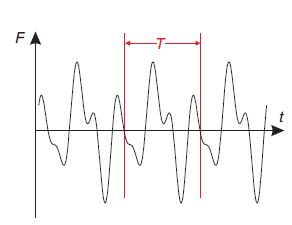
\includegraphics[height=50mm]{signal}}
	\hspace{5mm}
	\subfigure[]{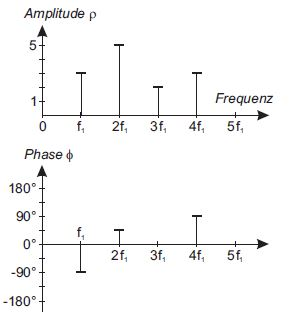
\includegraphics[height=50mm]{amplituden_phasenspektrum}}
	\caption{Periodisches Signal mit zugehörigem Amplituden- und Phasenspektrum (Quelle: Eichler))}
	\label{fig.Fourier}
\end{figure}
\\
Die Fouriertransformation überführt die Gleichung aus dem Zeitbereich $F(t)$ nun in den Frequenzbereich $F(\omega)$. Für analoge Signale ist die Fouriertransformation nun wie folgt definiert:
\begin{equation}
	\label{eq:Fouriertransformation}
	F(\omega) = \int\limits_{-\infty}^{\infty} x(t) e^\ind{-j\omega} \ind{d}t.
\end{equation}
\begin{equation}
	\label{eq:Inverse_Fouriertransformation}
	F(t) = \frac{1}{2\pi}\int\limits_{-\infty}^{\infty} F(\omega)e^\ind{j\omega} \ind{d}\omega
\end{equation}
Gleichung \ref{eq:Fouriertransformation} überführt eine von der Zeit abhängige Funktion aus dem Zeitbereich über Integration von $-\infty$ bis $\infty$ über alle Zeitpunkte $t$ in den Frequenzbereich. Die inverse Fouriertransformation wird durch Gleichung \ref{eq:Inverse_Fouriertransformation} beschrieben. Die Rücktransformation erfolgt durch Integration von $-\infty$ bis $\infty$ des von der Frequenz $\omega$ abhängigen Signals über alle Frequenzen $\omega$.

\section{Diskrete Fouriertransformation}
\label{sec.Diskrete Fouriertransformation}
% Quelle: Wendemuth
Die in Abschnitt \ref{sec:Fourierreihen und Fouriertransformation} dargestellten Gleichungen gelten für analoge Funktionen. In der Praxis ist es aber so, dass keine vollständige Kenntnis über ein Signal vorliegt, sondern dies nur durch Messungen zu diskreten Zeitpunkten abgetastet werden kann. Hieraus resultiert die Diskrete Fourier-Transformation (DFT). Die resultierenden Werte $F(n)$ der diskreten Fouriertransformation eines zu den Zeitpunkten $k$ abgetasteten Signals $f(t)$ können mittels Gleichung \ref{eq:DFT} berechnet werden. Die inverse diskrete Fouriertransformation erfolgt dann durch Gleichung \ref{eq:IDFT}.
\begin{equation}
	\label{eq:DFT}
	F(n) = \sum_{k=0}^{N-1}x[k]e^\ind{j\frac{2\pi}{N}kn}
\end{equation}
\begin{equation}
	\label{eq:IDFT}
	f[k] = \frac{1}{N}\sum_{k=0}^{N-1}F(n)e^\ind{j\frac{2\pi}{N}kn}
\end{equation} \\
Im Zusammenhang mit der Diskreten Fouriertransformation ist abschließend das Abtasttheorem von Nyquist und Shannon zu nennen. Das Theorem besagt, dass ein beliebig geformtes, kontinuierliches Signal immer dann durch ein diskretes Signal darstellbar und auch exakt wiederherstellbar ist, wenn die Abtastfrequenz des Signals mindestens doppelt so hoch ist, wie die höchste im kontinuierlichen Signal enthaltene Frequenz. Beträgt die höchste Frequenz in unserem Signal also beispielsweise \SI{10}{\Hz}, so müssen wir unser Signal mit mindestens \SI{20}{\Hz} abtasten, um unser Signal vollständig rekonstruieren zu können. \\
Die Folgen einer zu geringen Abtastfrequenz werden in \bild{Abtasttheorem} ersichtlich. Die Abtastung des Signals zu den mit schwarz markierten Zeitpunkten reicht nicht aus, um das in grau dargestellte Originalsignal zu rekonstruieren. Stattdessen ergibt sich das in rot dargestellte Signal.
\begin{figure}[!ht]
	\begin{center}
		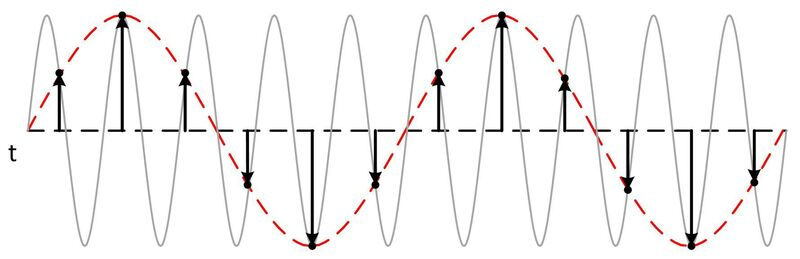
\includegraphics[height=50mm]{abtasttheorem}
		\caption{Originalsignal (grau) und durch Abtastung rekonstruiertes Signal (rot) Quelle(https://www.geothermie.de/bibliothek/lexikon-der-geothermie/a/abtasttheorem.html)}
		\label{fig.Abtasttheorem}
	\end{center}
\end{figure}
\section{Wahrscheinlichkeitsverteilungen}
\label{sec.Wahrscheinlichkeitsverteilungen}
\subsection{Binomialverteilung}
\label{sec.Binomialverteilung}
% Quelle: Teschl 2010
Als Bernoulli-Experiment wird ein Zufallsexperiment bezeichnet, bei dem es lediglich zwei Ausgänge geben kann. Ein Ereignis A tritt entweder ein oder nicht. Führt man ein Bernoulli-Experiment n-mal hintereinander unter den gleichen Bedingungen durch, so erhält man eine Bernoulli-Kette der Länge $n$. Das Eintreten des Ereignisses A wird gemeinhin als Erfolg bezeichnet, die Wahrscheinlichkeit $P(A)=p$ bezeichnet man als Erfolgswahrscheinlichkeit. Als Ereignis A kann hier beispielhaft das Werfen einer Münze mit dem Ausgang $Zahl$ genannt werden. Eine Binomialverteilung entsteht nun, wenn wir die Anzahl der Erfolge bei einer Bernoulli-Kette ermitteln wollen. Mathematisch formuliert lässt sich die Binomialverteilung ausdrücken als:
\begin{equation}
	\label{eq:Binomialverteilung}
	P(X=x) = \binom{n}{x}p^\ind{x} q^\ind{n-x}
\end{equation}\\
$X$ bezeichnet hierbei die Anzahl der Versuchsdurchführungen, bei denen ein Erfolg eintritt. $X$ kann die Werte $x = 0,1,2,\dots,n$ annehmen. $p$ steht für die Eintrittswahrscheinlichkeit eines Erfolges, $q$ für die Wahrscheinlichkeit eines Misserfolges. Die Zufallsvariable $X$ ist binomialverteilt und ihre Wahrscheinlichkeitsverteilung eine Binomialverteilung mit den Parametern $n,p$. Kurz: $X~Bi(n;p)$. Die grafische Darstellung einer Binomialverteilung für die Wahrscheinlichkeit der Anzahl an Würfen eines Würfels mit dem Ereignis 1 bei sieben Würfen ist in Abbildung xy abgebildet.
% Hier Bild aus Buch 2014 Mathe für Informatiker einfügen
% evtl noch Eigenschaften der Binomialverteilung einfügen? Oder unnötig?
\subsection{Poissonverteilung}
\label{sec.Poissonverteilung}
Eine Zufallsvariable $X$, welche unendlich viele Werte $x=0,1,2\dots$ mit den Wahrscheinlichkeiten
\begin{align}
	P(X=x) &= \frac{\lambda^\ind{x}}{x!} e^\ind{-\lambda} & (\lambda >0)
	\label{eq:Poisson Verteilung}
\end{align}
annehmen kann, wird als poissonverteilt mit dem Parameter $\lambda$ bezeichnet. Die zugehörige Verteilung heißt Poisson-Verteilung. Der Erwartungswert sowie die Varianz der Poisson-Verteilung werden ausgedrückt als:
\begin{align}
	\mu &= E(X) = \lambda \\
	\sigma^2 &= Var(X) = \lambda
	\label{eq:Poisson EW und Var}
\end{align}
Anhand der obigen Formeln erkennt man, dass der Parameter der Poisson-Verteilung grade gleich ihres Erwartungswertes ist, selbiges gilt für die Varianz.
Häufig ist es von Interesse, die Anzahl $X_t$ eines Ereignisses innerhalb eines Zeitraumes von 0 bis $t$ zu prognostizieren. Die Menge von Zufallsvariablen $X_t, t\geq 0,$ wird als Poisson-Prozess mit der Intensität $\lambda$ bezeichnet, falls $X_t$ einer Poisson-Verteilung folgt, es also gilt: \\
\begin{equation}
	P(X_t=x) = \frac{(\lambda t)^x}{x!} e^\ind{-\lambda t}
	\label{eq:Poisson-Prozess}
\end{equation}
Ein Poisson-Prozess muss dabei drei Voraussetzungen erfüllen:
\begin{itemize}
	\item Die Wahrscheinlichkeit für ein Ereignis ist proportional zur Beobachtungsdauer $\Delta t$, aber unabhängig von der Lage der Beobachtungsdauer.
	\item Die Wahrscheinlichkeiten für ein Ereignis an unterschiedlichen Orten sind voneinander unabhängig
	\item Für infinitesimal kleine $\Delta t$ ist die Wahrscheinlichkeit, dass das Ereignis mehr als einmal auftritt, im Vergleich zur Wahrscheinlichkeit, dass es genau einmal vorkommt, vernachlässigbar klein.
\end{itemize}



    	\chapter{Stand der Technik}
% Ersten Satz noch ändern nachdem das Kapitel fertig ist.
% Schauen, dass eine konsistente Schreibweise benutzt wird. Also z.B. einheitliches Wort für "Umweltzustand", oder was auch immer ich dafür wähle.
% Ereignis und Umweltzustand werden irgendwie gleich benutzt.
%In diesem Kapitel wird auf den Stand der Technik eingegangen. Im weitesten zitiere ich %hier die wissenschaftlichen Paper, auf denen meine Arbeit beruht. Ob man das Kapitel %noch weiter einteilen muss, wird sich später zeigen, erstmal lasse ich es ohne %Unterkapitel. \\
Mobile Roboter finden immer mehr Einzug in Umgebungen, welche von Menschen bewohnt sind. Diese Menschen üben Aktivitäten aus, welche in der Folge zu Veränderungen eben dieser Umgebung führen. Man kann davon ausgehen, dass viele dieser Aktivitäten täglichen Routinen mit typischen Mustern folgen, welche von mobilen Robotern erkannt werden und zur robusteren Darstellung ihrer Umgebung genutzt werden können. Mapping in statischen Umgebungen stellt ein weit erforschtes Gebiet dar \cite{Eichler.2006}.
% Ist Mapping das richtige Wort, oder vllt. doch lieber ein deutsches Pendant finden? 
Für das Mapping, also die Kartierung dynamischer Umgebungen gibt es verschiedene Ansätze. Während ein Ansatz darauf abzielt, sich bewegende Objekte aus der Umgebungsdarstellung herauszufiltern \cite{Hahnel.2002}, werden in anderen diese Objekte getrackt und als bewegte Landmarken klassifiziert \cite{Montesano.2008}. Diese separations-basierten Ansätze können jedoch nicht auf Langzeitveränderungen der Umgebungsstruktur reagieren. \\
Im Gegensatz hierzu stehen adaptive Ansätze, welche davon ausgehen, dass der Prozess der Kartierung niemals komplett abgeschlossen ist und diesen durch kontinuierliches Mapping aktualisieren. So können der Karte durch neue Observierungen des mobilen Roboters neue Features hinzugefügt werden 
\cite{Milford.2010}. In \cite{Krajnik.2014} wird nun erstmalig versucht, die räumlich-zeitliche Dynamik einer Umgebung durch ihr Frequenzspektrum darzustellen. Die Werte von lokalen Umweltzuständen, wie zum Beispiel einer Tür, welche entweder offen oder geschlossen sein kann, sollen anhand von Wahrscheinlichkeitsfunktionen repräsentiert werden, welche aus der Superposition periodischer Funktionen resultieren. In \cite{Krajnik.2014} wird als Motivation dazu angeführt, dass bei den meisten Mapping-Ansätzen wichtige Umweltzustände lediglich statisch durch zwei eindeutige Zustände dargestellt werden. Eine Tür ist also entweder dauerhaft geöffnet oder geschlossen. % Hier noch eine entsprechende Quelle einfügen.\\
Diese Zustände können jedoch auch durch ihre Wahrscheinlichkeit $p_j$ ausgedrückt werden. Bayes-Filter gehen hierzu von einer statischen Welt aus, d.h. die Wahrscheinlichkeiten der Zustände $p_j$ werden als konstant angesehen. Durch neue Beobachtungen können diese konstanten Annahmen verändert werden, alte Beobachtungen werden so jedoch über die Zeit "vergessen" \cite{Krajnik.2014}. Nimmt man nun jedoch an, dass diese Zustandswahrscheinlichkeiten Funktionen der Zeit sind, also $p_j (t)$ gilt, und diesen zeitlichen Veränderungen der Wahrscheinlichkeiten eine finite Nummer periodischer Prozesse zu Grunde liegt, so könnte man den Einfluss und die Periodizität eben dieser Prozesse identifizieren und die Zustandswahrscheinlichkeit $p_j (t)$ aus dieser Beschreibung ermitteln. In \cite{Krajnik.2014} wird nun die in Abschnitt \ref{sec:Fourierreihen und Fouriertransformation} erläuterte Fouriertransformation benutzt, um diese periodischen Prozesse zu identifizieren. Als Beispiel wird ein Belegungsnetz herangeführt. Jede der Zellen des Belegungsnetzes kann zwei Zustände $s_j = \{frei, belegt\}$ annehmen. Diese Zustände sind jedoch nicht konstant, sondern eine Funktion der Zeit, also $s_j (t)$. Die Unsicherheit des Zustandes wird nun durch sein Wahrscheinlichkeit $p_j (t)$ ausgedrückt. Da die Zellen unabhängig voneinander sind, kann die Fouriertransformation separat auf jede Zelle des Belegungsnetzes angewendet werden. \\ Die über die Zeit aufgetragenen Zustände einer Zelle $s(t)$ werden mittels der Fouriertransformation $P = FT(s(t))$ transformiert. Es werden \textit{l} Koeffizienten $P_i$ des Spektrums $P$ ausgewählt und zusammen mit ihren Frequenzen $\omega_i$ benutzt, um mittels der inversen Fouriertransformation $p(t) = IFT(s(t))$ die Wahrscheinlichkeitsfunktion $p(t)$ des Zellzustandes zu bestimmen. Abschließend wird ein Schwellwert benutzt, um aus $p(t)$ eine Schätzung $s'(t)$ der tatsächlichen Zustandsfunktion $s(t)$ zu bestimmen. Das Set $P$ besteht hierbei aus $l$ Tripeln mit den Einträgen $(abs(P_i), arg(P_i), \omega_i)$, wobei $abs(P_i)$ für die Amplitude, $arg(P_i)$ für den Phasenversatz und $\omega_i$ für die Frequenz des jeweiligen periodischen Prozesses steht, welcher den Zustand $s(t)$ beeinflusst. \\

Der Zustand einer Zelle wird nun über die Gleichung \ref{eq:Zellzustand} approximiert: 
\begin{equation}
	s(t) = (IFT(P) > 0.5) \oplus  (t \notin 0)
	\label{eq:Zellzustand}
\end{equation}
Ist die Wahrscheinlichkeit $p(t)$ einer Zellbelegung größer als 0.5, so wird die Zelle als belegt geschätzt.
% sofern der Zeitpunkt $t$ nicht zum Set der Ausreißer 0 gehört.
% Ausreißer-Set muss noch eingebunden werden.
% evlt. ist Ausreißer-Set für mich garnicht so relevant, da FreMEn das Modell ja automatisch aktualisiert
Der in Gleichung \ref{eq:Zellzustand} benutzte Schwellwert von 0.5 kann willkürlich gesetzt werden. So können Vorhersagen über zukünftige Zustände der Zelle mit einem gewissen Konfidenzniveau von $c$ durch die Gleichung:
\begin{equation}
	s'(t,c) = IFT(P) > c
	\label{eq:Zustandsvorhersage}
\end{equation}
getroffen werden. Grafisch verdeutlicht wird die Methodik durch \bild{FreMEn Beispiel}. 

\begin{figure}[!ht]
	\begin{center}
		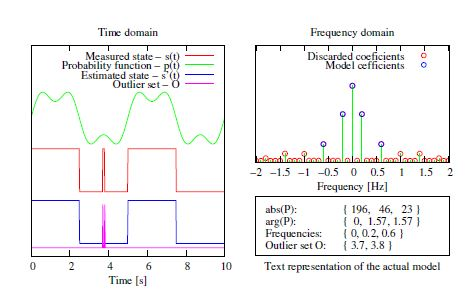
\includegraphics[]{Abbildungen/stand_der_technik/example_of_measured_state_and_prediction}
		\caption{Beispiel eines über die Zeit gemessenen Zellzustandes sowie seines Spektralmodells und Wahrscheinlichkeitsprädiktion Quelle \cite{Krajnik.2014}}
		\label{fig.FreMEn Beispiel}
	\end{center}
\end{figure}
% Wieso ist das Bild nicht an der eingegebenen Stelle?
In der linken Grafik rot dargestellt sind die über einen zeitlichen Verlauf aufgenommenen, binären Zustände einer Beispielzelle. Der grüne Graph beschreibt das zugehörige FreMEn-Modell der Ordnung drei. In blau aufgetragen sind die Vorhersagen des Modells, ermittelt anhand eines Schwellwertes von 0.5. Der lila Graph stellt die Zeitpunkte dar, zu denen die Modellvorhersage von den tatsächlichen Zellzuständen abweicht \cite{Krajnik.2014}. Die rechte obere Grafik repräsentiert das Frequenzspektrum der Zelle, die für das Modell ausgewählten Frequenzen sind durch blaue Kreise markiert. Das zuvor erwähnte Tripel bestehend aus Amplitude, Phasenversatz und Frequenz der jeweiligen periodischen Prozesse ist in der rechten unteren Grafik dargestellt. Um die Auswirkungen des Modellgrades, also der Anzahl der in das Modell einfliessenden periodischen Prozesse, zu erforschen, wurde die Methodik auf einen Datensatz angewendet, bei welchem ein mobiler SCITOS-G5 Roboter, ausgestattet mit RGB-D und Lasersensoren, Personen in einem Bürogebäude über eine Dauer von einer Woche mit einer Rate von \SI{30}{\hertz} detektiert hat. \\
Die Genauigkeit des Modells $q(t_a,t_b)$ wird anhand von Gleichung \ref{eq:Modellgenauigkeit} berechnet und beschreibt das Verhältnis von korrekt geschätzten Zellzuständen zu der Gesamtdauer des betrachteten Intervalls:
\begin{equation}
	q(t_a,t_b) = \frac{1}{t_b - t_a} \int_{t_a}^{t_b} |s'(t) - s(t)| \ind{d}t
	\label{eq:Modellgenauigkeit}
\end{equation}
Unterschieden wurde nun in \cite{Krajnik.2014} zwischen dem Rekonstruktionsfehler $q_r$ sowie dem Prädiktionsfehler $q_p$. Der Rekonstruktionsfehler beschreibt, wie genau das Modell Zeitintervalle beschreibt, welche zur Ermittlung der Modellparameter verwendet wurden. Der Prädiktionsfehler hingegen beschreibt die Genauigkeit des Modells in Bezug auf Zeiträume, welche nicht zur Modellermittlung verwendet wurden. Die ermittelte Abhängigkeit des Rekonstruktions-sowie Prädiktionsfehlers von der Modellordnung ist in \bild{fig.predict_reconstruct_error} aufgezeigt. Hierbei erfolgte die Berechnung des Modells und des Rekonstruktionsfehlers $q_r$ anhand eines einwöchigen Datensatzes, die Evaluierung des Modells und die Ermittlung des Prädiktionsfehlers $q_p$ wurde mittels zwei externer Tage durchgeführt.  \\
% Wieso hat die Grafik so hässliche graue Ränder?
\begin{figure}[!ht]
	\begin{center}
		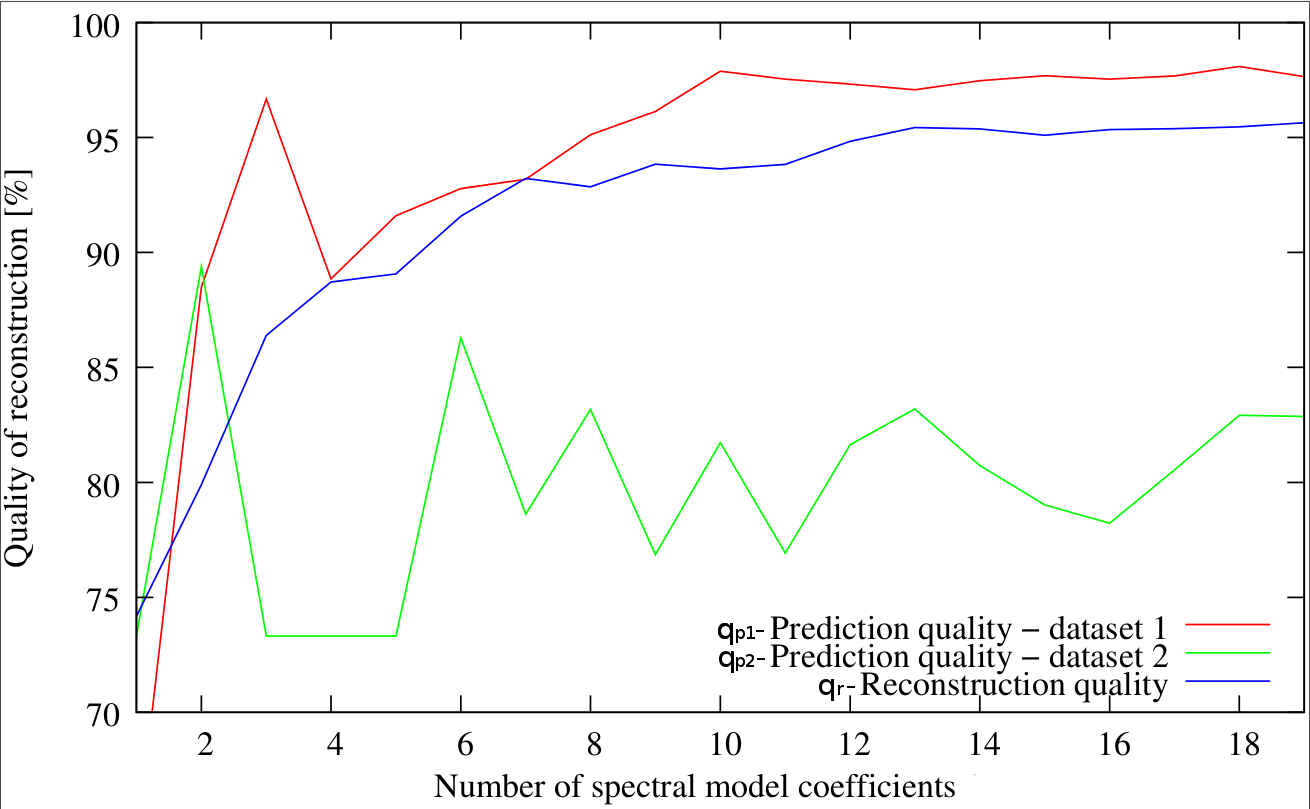
\includegraphics[width=0.7\linewidth]{Abbildungen/stand_der_technik/predict_reconstruct_error}
		\caption{Modellgenauigkeit vs. Modellordnung Quelle \cite{Krajnik.2014}}
		\label{fig.predict_reconstruct_error}	
	\end{center}
	
\end{figure}


Die Rekonstruktionsgenauigkeit liegt bei einer Modellordnung von 15, d.h. es wurden 15 periodische Prozesse zum Approximieren des Zustandssignales verwendet, bei 95 \%. Die Rekonstruktionsgenauigkeit $q_r$ steigt dabei monoton mit der Modellordnung, die Prädiktionsgenauigkeit $q_p$ hingegen nicht. 
% Manchmal nenne ich q_p hier Prädiktionsgenauigkeit und manchmal Fehler, das muss ich noch einheitlich machen. 
\\
Die lokalen Maxima von $q_\ind{p1}$ und $q_\ind{p2}$ lassen den Schluss zu, dass für die Vorhersage eine Modellordnung von zwei oder drei optimal ist (siehe \bild{predict_reconstruct_error}). \\
% \cite{Krajnik.2015b} 
Einen Vergleich zwischen der in \cite{Krajnik.2014} beschriebenen "Frequency Map Enhancement" Methode (FreMEN) und der Anwendung von periodischen Gauß-Mixmodellen zur Darstellung der Dynamik von Umweltzuständen zieht \cite{Krajnik.2015b}. FreMEn basiert hier, wie auch schon in \cite{Krajnik.2014} auf der Idee, die zeitliche Funktion $s(t)$ eines Umweltzustandes durch seine Wahrscheinlichkeitsfunktion $p(t)$ zu schätzen. Auch hier wird wieder mittels einer Fouriertransformation das Frequenzspektrum $S(\omega)$ der zeitlichen Funktion $s(t)$ bestimmt, und die \textit{l} prominentesten Frequenzen mit ihren Amplituden $a_j$, ihrem Phasenversatz $\varphi_j$ sowie ihrer Frequenz $\omega_j$ abgespeichert. Die Ermittlung der Wahrscheinlichkeit eines Umweltzustandes zum Zeitpunkt \textit{t} ergibt sich nun durch die Superposition der \textit{l} Frequenzen mittels Gleichung (\ref{eq:Superposition}):
\begin{equation}
	p(t) = a_0 + \sum_{j=1}^{n} a_j \cos(\omega_j t + \varphi_j)
	\label{eq:Superposition}
\end{equation}
Die erste spektrale Komponente $a_0$ stellt hierbei den Durchschnitt aller binären Werte von $s(t)$, also dessen Gleichanteil (siehe Abschnitt \ref{sec:Fourierreihen und Fouriertransformation}) dar. FreMEn besitze aber laut \cite{Krajnik.2015b} zwei wesentliche Nachteile. So erlaube es zum einen lediglich einen periodischen Prozess pro Frequenz zu modellieren. Des Weiteren bilde es wiederkehrende, aber kurze Prozesse, schlecht ab. Als Beispiel wird hier die morgendliche Dusche angeführt, welche eine tägliche, aber kurze Routine sei. Da in \cite{Krajnik.2014} herausgearbeitet wurde, dass die optimale Modellordnung für eine möglichst genaue Prognostizierfähigkeit bei einer Größe von lediglich zwei bis drei liegt, könnten solche kurzen Routinen schlicht nicht abgebildet werden. \\ Als zweiter Ansatz werden Gaussian Mixture Models (GMM) genannt. Diese können multidimensionale Funktionen als gewichtete Summe aus mehreren Gauß-Funktionen mittels Gleichung (\ref{eq:Gaussian_Mixture_Models}) approximieren:
\begin{equation}
	f(t) = \frac{1}{\sqrt{2 \pi}} \sum_{j=1}^{m} \frac{\omega_j}{\sigma_j} e^\ind{- \frac{(t- \mu_j)^2}{2 \sigma_j ^2}}
	\label{eq:Gaussian_Mixture_Models}
\end{equation}
Die Parameter der individuellen Komponenten eines GMM, namentlich das Gewicht $\omega_j$, der Durchschnitt $\mu_j$ sowie die Standardabweichung $\sigma_j$ werden typischerweise mittels Trainingsdaten anhand des Iterative Expectation Maximization (EM) oder des Maximum A-Posteriori (MAP) Algorithmus ermittelt. Während GMM's in der Lage sind, Funktionen jeglichen Aussehens zu modellieren, liegt ihre Limitation darin, dass sie definitionsgemäß keine periodischen Funktionen repräsentieren können \cite{Krajnik.2015b}. Um diesem Problem entgegenzuwirken, wird vorab eine Periodendauer von einem Tag vorgegeben. Diese Vorgabe erlaubt es, die gemessene Sequenz der Umweltzustände $s(t)$  in eine Sequenz $p'(t)$ umzuwandeln:
\begin{equation}
	p'(t) = \frac{k}{\tau} \sum_{i=1}^{\frac{k}{\tau}} s(t+i \tau)
	\label{eq:GMM_sequence}
\end{equation}
In Gleichung (\ref{eq:GMM_sequence}) bezeichnet $\tau$ die vorab definierte Periodendauer, $k$ beschreibt die Länge der Sequenz $s(t)$. Nach Anwendung des Expectation Maximization Algorithmus kann nun die Wahrscheinlichkeit für einen Umweltzustand mittels Gleichung \ref{eq:Gauss_Probability} berechnet werden: 
\begin{equation}
	p(t) = \frac{1}{\sqrt{2 \pi}} \sum_{j=1}^{m} \frac{w_j}{\tau_j} e ^\ind{- \frac{(mod(t,\tau) - \mu_j)^2}{2 \sigma_j^2}}
	\label{eq:Gauss_Probability}
\end{equation}
Hierbei beschreibt $\tau$ die vorgegebene Periodendauer der Funktion $p(t)$ und $mod$ ist der Modulo-Operator. Dass die Stärken und Schwächen dieser periodischen GMM-basierten (PerGaM) Modelle komplementär zu jenen der FreMEn-Methodik sind, wir anhand von \bild{PerGaM_vs_FreMEn} deutlich.
\begin{figure}[!ht]
	\begin{center}
		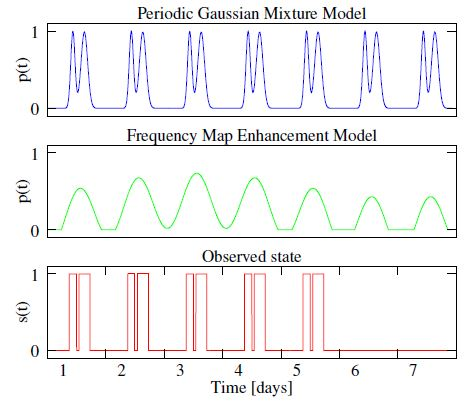
\includegraphics[]{Abbildungen/stand_der_technik/PerGaM_vs_FreMEn}
		\caption{PerGaM und FreMEn Modellvergleich Quelle \cite{Krajnik.2015b}}
		\label{fig.PerGaM_vs_FreMEn}
	\end{center}
\end{figure}
Das PerGaM-Modell kann selbst kurze, mehrfach auftretende Routinen approximieren, jedoch kann es lediglich eine Periodendauer repräsentieren, welche a priori bekannt bzw. festgelegt werden muss. Als Resultat werden kurzzeitige Routinen, wie z.B. Mittagspausen, gut approximiert, die wöchentliche Dynamik mit dem Fehlen von Personen am Wochenende kann hingegen jedoch nicht modelliert werden. Im Vergleich dazu sieht man das FreMEn-Modell, welches diese Wochendynamik durch ein Abflachen der Signalamplitude an den beiden Wochenendtagen abbildet (siehe \bild{PerGaM_vs_FreMEn}). \\
In Bezug auf die zeitlich-räumliche Kartierung durch mobile Roboter führt \cite{Krajnik.2015} an, dass dies auch eine räumlich-zeitliche Explorationsstrategie benötigt. Im Vergleich zu klassischen Explorationsstrategien, bei denen, bedingt durch die endliche Größe der zu erforschenden Karte, die Exploration ebenfalls finit ist, sei die Exploration dynamischer Umgebungen niemals abgeschlossen. Vielmehr bekäme die räumlich-zeitliche Exploration Teil der täglichen Routine des Roboters.
Es stellt sich ein wesentlicher Nachteil der in \cite{Krajnik.2014} vorgestellten Methode zur Darstellung von Umweltzuständen in Bezug auf die kontinuerliche Exploration einer Karte durch einen mobilen Roboter heraus. Diese beruht auf der traditionellen Fast Fourier Transformation (FFT). Die Fast Fourier Transformation kann jedoch lediglich die komplette Sequenz eines Umweltzustandes $s(t)$ in sein Frequenzspektrum $S(\omega)$ transformieren. Außerdem erfordert der Algorithmus, dass die Zustandsobservierungen mit der immer gleichen Frequenz aufgenommen werden.  Orte mit der immer selben Frequenz zu erkunden, sei jedoch nicht effizient, sodass in \cite{Krajnik.2015} eine neue Methode zur Darstellung von Umweltzuständen durch zeitlich variable Wahrscheinlichkeitsfunktionen vorgestellt wird. Die Methode erlaubt ein inkrementelles und kontinuierliches Aktualisieren des räumlich-zeitlichen Umgebungsmodells durch wenige Observierungen, welche zu unterschiedlichen, nicht gleichmäßig verteilten Zeitpunkten, und an unterschiedlichen Orten aufgenommen werden können. \\
Jeder Umweltzustand wird nun durch die Nummer getätigter Observierungen $n$, seines Durchschnittes $\mu$ sowie zwei Sets $A,B$ komplexer Zahlen $\alpha_k$ und $\beta_k$, welche zu dem Set $\Omega$ periodischer Prozesse $\omega_k$ gehören, die den Umweltzustand beeinflussen, beschrieben. Anfangs wird der Wert $\mu$ jedes Umweltzustandes zu 0.5 und alle $\alpha_k$ sowie $\beta_k$ zu 0 gesetzt, was einem vollkommen unbekannten Zustand entspricht. Die inkrementelle Aktualisierung des Modells erfolgt nun anhand der Gleichungen (\ref{eq:mu_Aktualisierung}) - (\ref{eq:Update_step_FreMEn}):
\begin{align}
	\label{eq:mu_Aktualisierung}
	\mu &\leftarrow \frac{1}{n+1}(n \mu + s(t)), \\
	\alpha_k &\leftarrow \frac{1}{n+1} (n \alpha_k + s(t) e^\ind{-jt\omega_k})  &\forall \omega_k \in \Omega, \\
	\beta_k &\leftarrow \frac{1}{n+1} (n \beta_k + \mu e^{ind{-jt\omega_k}})  &\forall \omega_k \in \Omega, \\
	n &\leftarrow n + 1
	\label{eq:Update_step_FreMEn}
\end{align}
Die schrittweise Aktualisierung entspricht dabei einer inkrementellen Mittelwertbildung. Der Betrag $\gamma_k = |\alpha_k - \beta_k|$ entspricht hierbei dem durchschnittlichen Einfluss des periodischen Prozesses $k$ auf den Umweltzustand $s(t)$.
Wären die Zeitpunkte der Observationen $t$ und die Frequenzen $\omega_k$ gleichmäßig verteilt, also $t=i\Delta_t$ und $\omega_k = i\Delta_\ind{\omega}$, so entsprächen die obigen Formeln der diskreten Fouriertransformation.
Um den zukünftigen Wert eines Umweltzustandes prognostizieren zu können, werden nun wie auch in \cite{Krajnik.2014} die $m$ periodischen Prozesse mit den höchsten absoluten Werten $|\gamma_k|$ ausgewählt. Die Wahrscheinlichkeit eines Umweltzustandes wird dann mittels:
\begin{equation}
	p(t) = \varsigma(\mu + \sum_{l=1}^{m} |\gamma_l|\cos(\omega_k t + arg(\gamma_l)))
	\label{eq:State_probability}
\end{equation}
berechnet. Die Funktion $\varsigma(.)$ sorgt dafür, dass $p(t) \in [0,1]$. Der optimale Wert für $m$ wird wie schon in \cite{Krajnik.2014} so gewählt, dass der Prädiktionsfehler $q_p$ minimiert wird. \\
Eine weitere Methodik zur Modellierung von Umweltzuständen wird in \cite{Jovan.2016} vorgestellt. Die hier genannte Methode beruht auf der Kombination von zeitveränderlichen Poisson-Prozessen und einer Frequenzanalyse. Die Häufigkeit des Auftretens eines Ereignisses innerhalb eines Zeitintervalls wird gezählt. Somit kann die Darstellung des simplen Auftretens- bzw. Nichtauftretens eines Umweltzustandes \cite{Krajnik.2014} um dessen \glqq Intensität\grqq{} erweitert werden. Zur Modellierung dieser Aktivitäten wird das Vorhandensein von Umweltzuständen mit Hilfe von Poisson-Prozessen modelliert. Wie schon  in Abschnitt \ref{sec.Poissonverteilung} beschrieben, wird auch hier die Poisson-Verteilung mittels:
\begin{equation}
	P(N;\lambda) = \frac{e^\ind{-\lambda} \lambda^N}{N!}	N=0,1,2,\dots
\end{equation}
\begin{align}
	P(N;\lambda) = \frac{e^\ind{-\lambda} \lambda^N}{N!}	N=0,1,2,\dots
\end{align}

wobei $P(N;\lambda)$ die Wahrscheinlichkeit $P$ für den Fall beschreibt, dass innerhalb eines Zeitintervalls $\Delta t$ mit einer durchschnittlichen Aktivitätenanzahl von $\lambda$ exakt $N$ Aktivitäten vorkommen. Die Daten in \cite{Jovan.2016} wurden von einem mobilen Metralabs Scitos A5-Roboter aufgenommen, welcher sich, ausgestattet mit einem robusten Personen-Tracking-Algorithmus, einen Monat lang in einem Bürogebäude bewegte. Die Abhängigkeit der durchschnittlichen Aktivitätenanzahl $\lambda$ vom betrachteten Zeitintervall wird durch $\lambda (t_i, t_j)$ ausgedrückt, wobei  $t_i$ den Anfangszeitpunkt und $t_j$ den Endzeitpunkt des Intervalls beschreibt. Da die von dem Roboter aufgenommenen Daten nur einen kleinen Teil der Gesamtheit an Aktivitäten repräsentiert, wird $\lambda$ mittels einer Konfidenz-basierten Schätzung bestimmt. Der Poisson-Parameter $\lambda$ folgt hierbei einer Gammaverteilung:
\begin{equation}
	\lambda \sim \Gamma(\lambda ; \alpha, \beta)
\end{equation}
Die a-posteriori Wahrscheinlichkeit für $\lambda (t_i, t_j)$ berechnet sich unter Berücksichtigung der aufgenommenen Daten nun zu:
\begin{equation}
	P(\lambda | x_1, \dots, x_n) = \Gamma(\lambda, \alpha + \sum_{i=1}^{n} x_i, \beta +n)
\end{equation}
wobei $x_1, \dots , x_n$ die im betreffenden Intervall aufgezeichneten Daten bezeichnet, der Parameter $\alpha$ steht für den Formfaktor, $\beta$ für den inversen Skalenparameter der Gammaverteilung.
% Hier dann noch das Paper von Marvin zitieren, wo die Bestimmung von alpha und beta deutlich anschaulicher und inkrementell beschrieben wird. 
Der Datensatz wird in Wochen eingeteilt, für ein Zeitintervall wird eine Dauer von zehn Minuten gewählt. Die Maximum a posteriori-Wahrscheinlichkeit (MAP) jedes Parameters $\lambda(t_i, t_j)$ wird als Punktschätzung für $\lambda$ gewählt. Die Verknüpfung sämtlicher Punktschätzungen über den definierten Zeitraum einer Woche ergibt das Poisson-Prozess-Model, welches in \bild{poisson-prozess-model1} grafisch aufgezeichnet ist. 
\begin{figure}[!ht]
	\begin{center}
		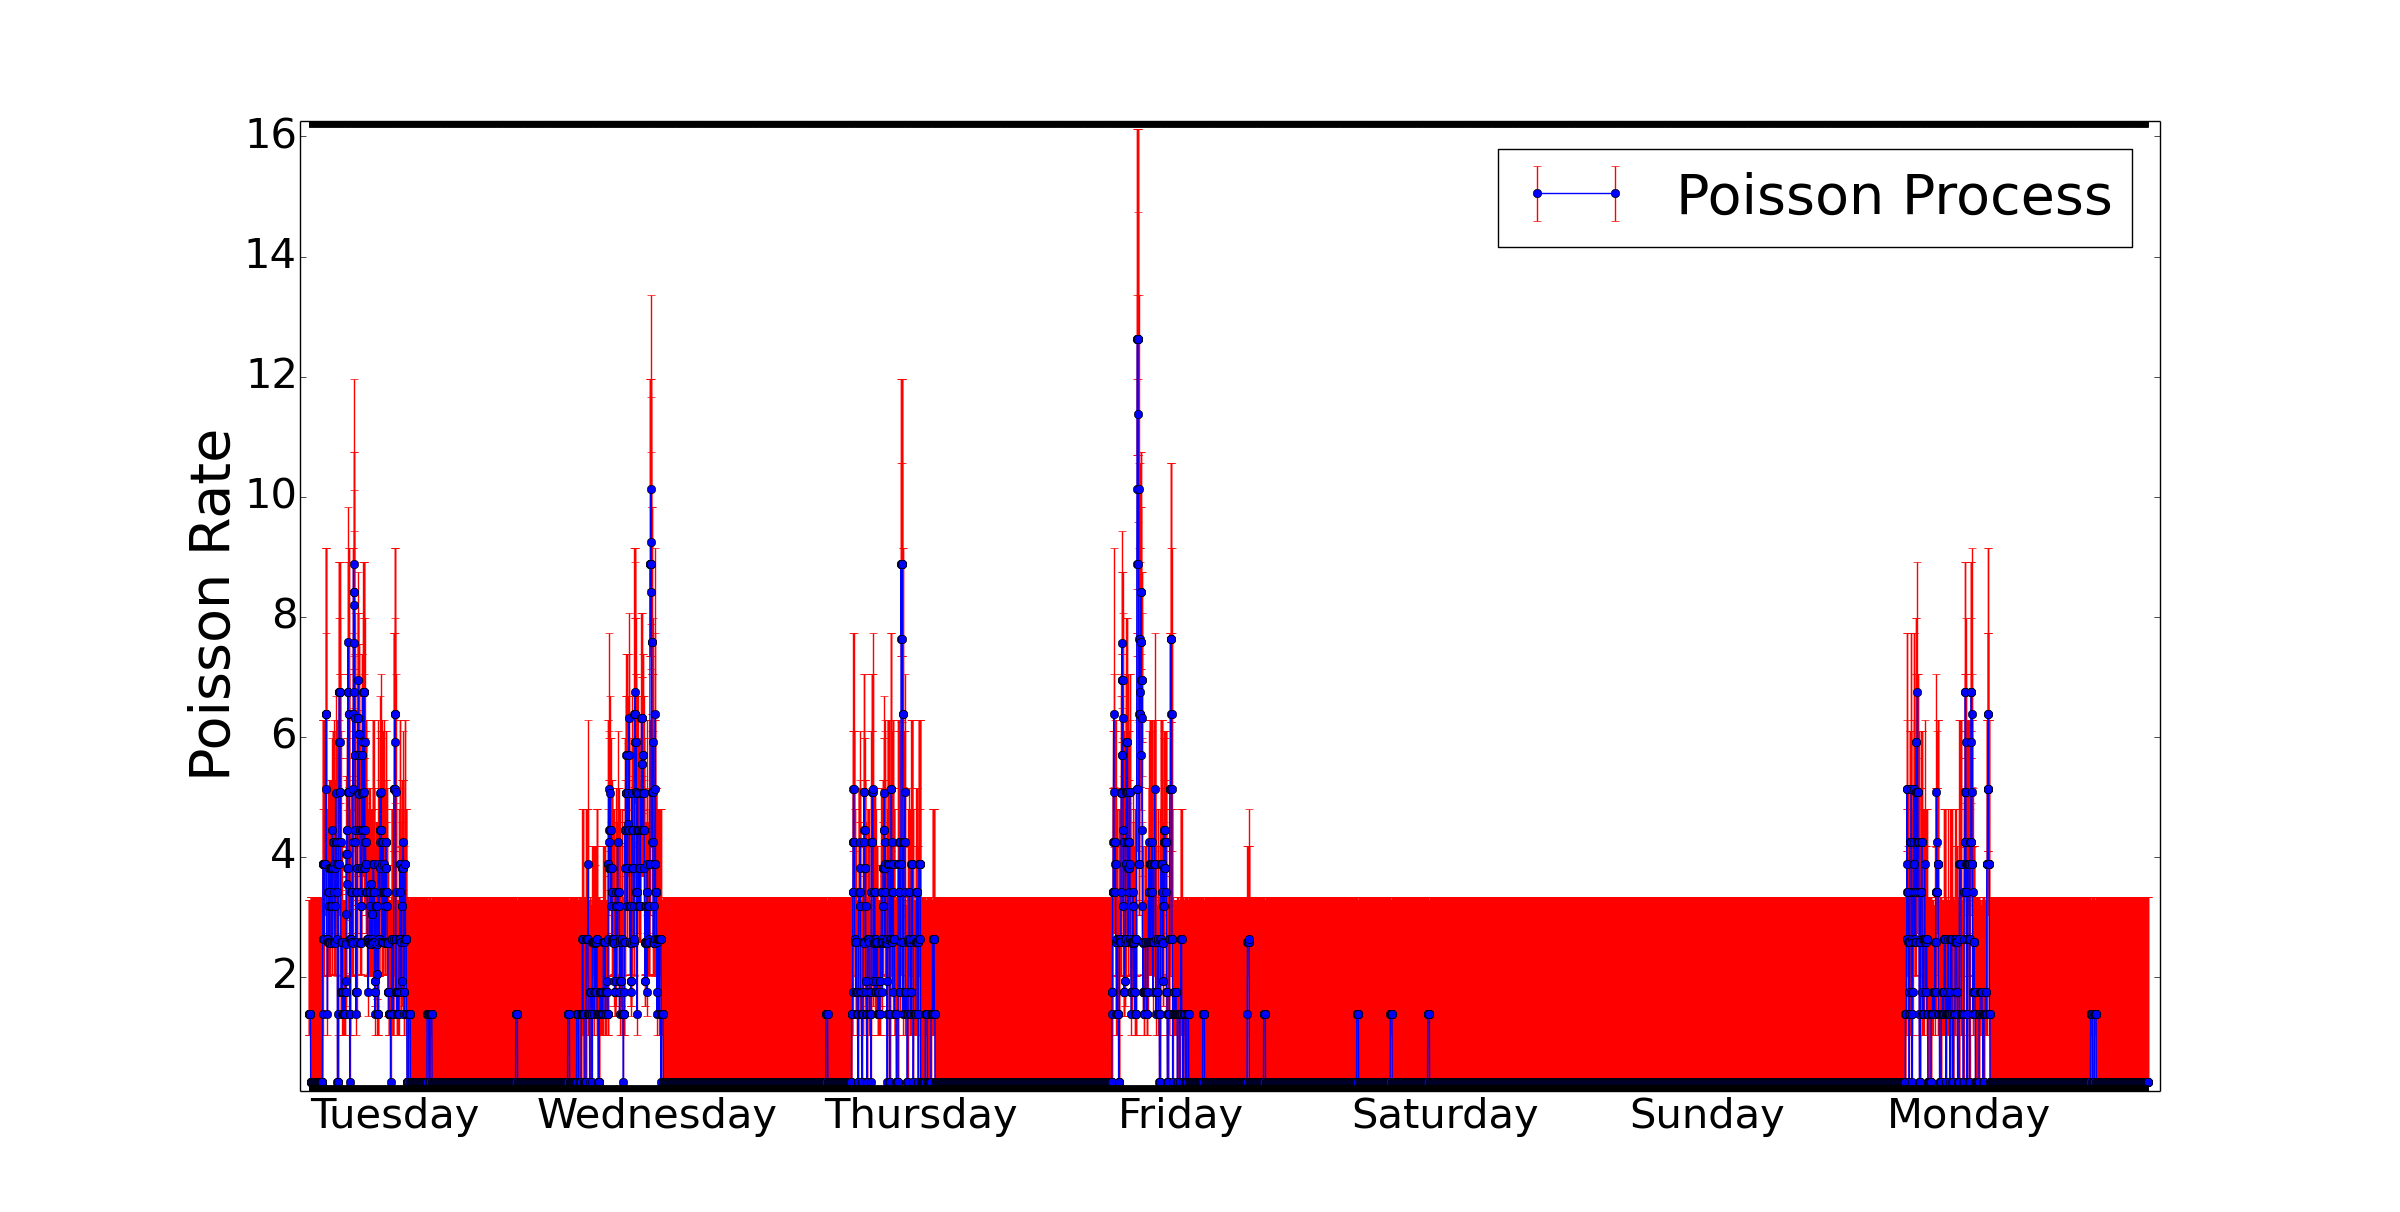
\includegraphics[width=0.7\linewidth]{Abbildungen/stand_der_technik/poisson-prozess-model1}
		\caption{Aktivitätsraten $\lambda$ des Poisson-Prozess-Modells ermittelt anhand eines 4 Wochen Zeitraumes Quelle \cite{Jovan.2016}}
		\label{fig.poisson-prozess-model1}
	\end{center}
\end{figure}

Für jedes $\lambda$ wurden die Daten von vier aufeinanderfolgenden Wochen verwendet, die roten Schranken zeigen die oberen und unteren Grenzen des Konfidenzintervals für jedes $\lambda$. \\
Nach der Berechnung des Poisson-Prozess-Modells wird nun die Fouriertransformation auf $\lambda (t)$ angewendet. Ebenso wie in \cite{Krajnik.2014} werden die $l$ Frequenzen mit den höchsten Amplituden zur Konstruktion von $\lambda' = IFT(F'(\omega))$ verwendet. Im Gegensatz zu der in \cite{Krajnik.2014} verwendeten und hier als \textit{l Best Amplitude Model (BAM)} bezeichneten Methode wird in \cite{Jovan.2016} die \textit{l Addition Amplitude Model (AAM)} Methode verwendet. Es wird angeführt, dass das \textit{BAM} den Betrag des Original-Signals nicht komplett abbilden kann, sofern die Sampling-Rate der Daten deutlich höher ist als die höchste beobachtete Frequenz. \\ \textit{AAM} hingegen berechnet das Fourierspektrum des Poisson-Prozess-Modells, findet die Frequnz $\omega_k$ mit der höchsten Amplitude und zieht es von den Daten ab. Die modifizierten Daten werden wieder transformiert und das Frequenzspektrum erneut berechnet. Findet sich in diesem Frequenzspektrum eine bereits vorher identifizierte Frequenz, so wird dessen neuerliche Amplitude auf die bereits vorhandene addiert, und die Daten erneut modifiziert. Dieses Vorgehen wird bis zur Identifikation der \textit{l} Frequenzen mit den höchsten Amplituden wiederholt. \bild{BAM_AAM_Vergleich} bietet einen Vergleich von den beiden Methoden zur Abbildung des Poisson-Prozess-Modells. Aus der Grafik wird ersichtlich, dass das \textit{AAM} die Beträge des Original-Modells deutlich besser abbilden kann als das \textit{BAM}.

\begin{figure}[!ht]
	\centering
	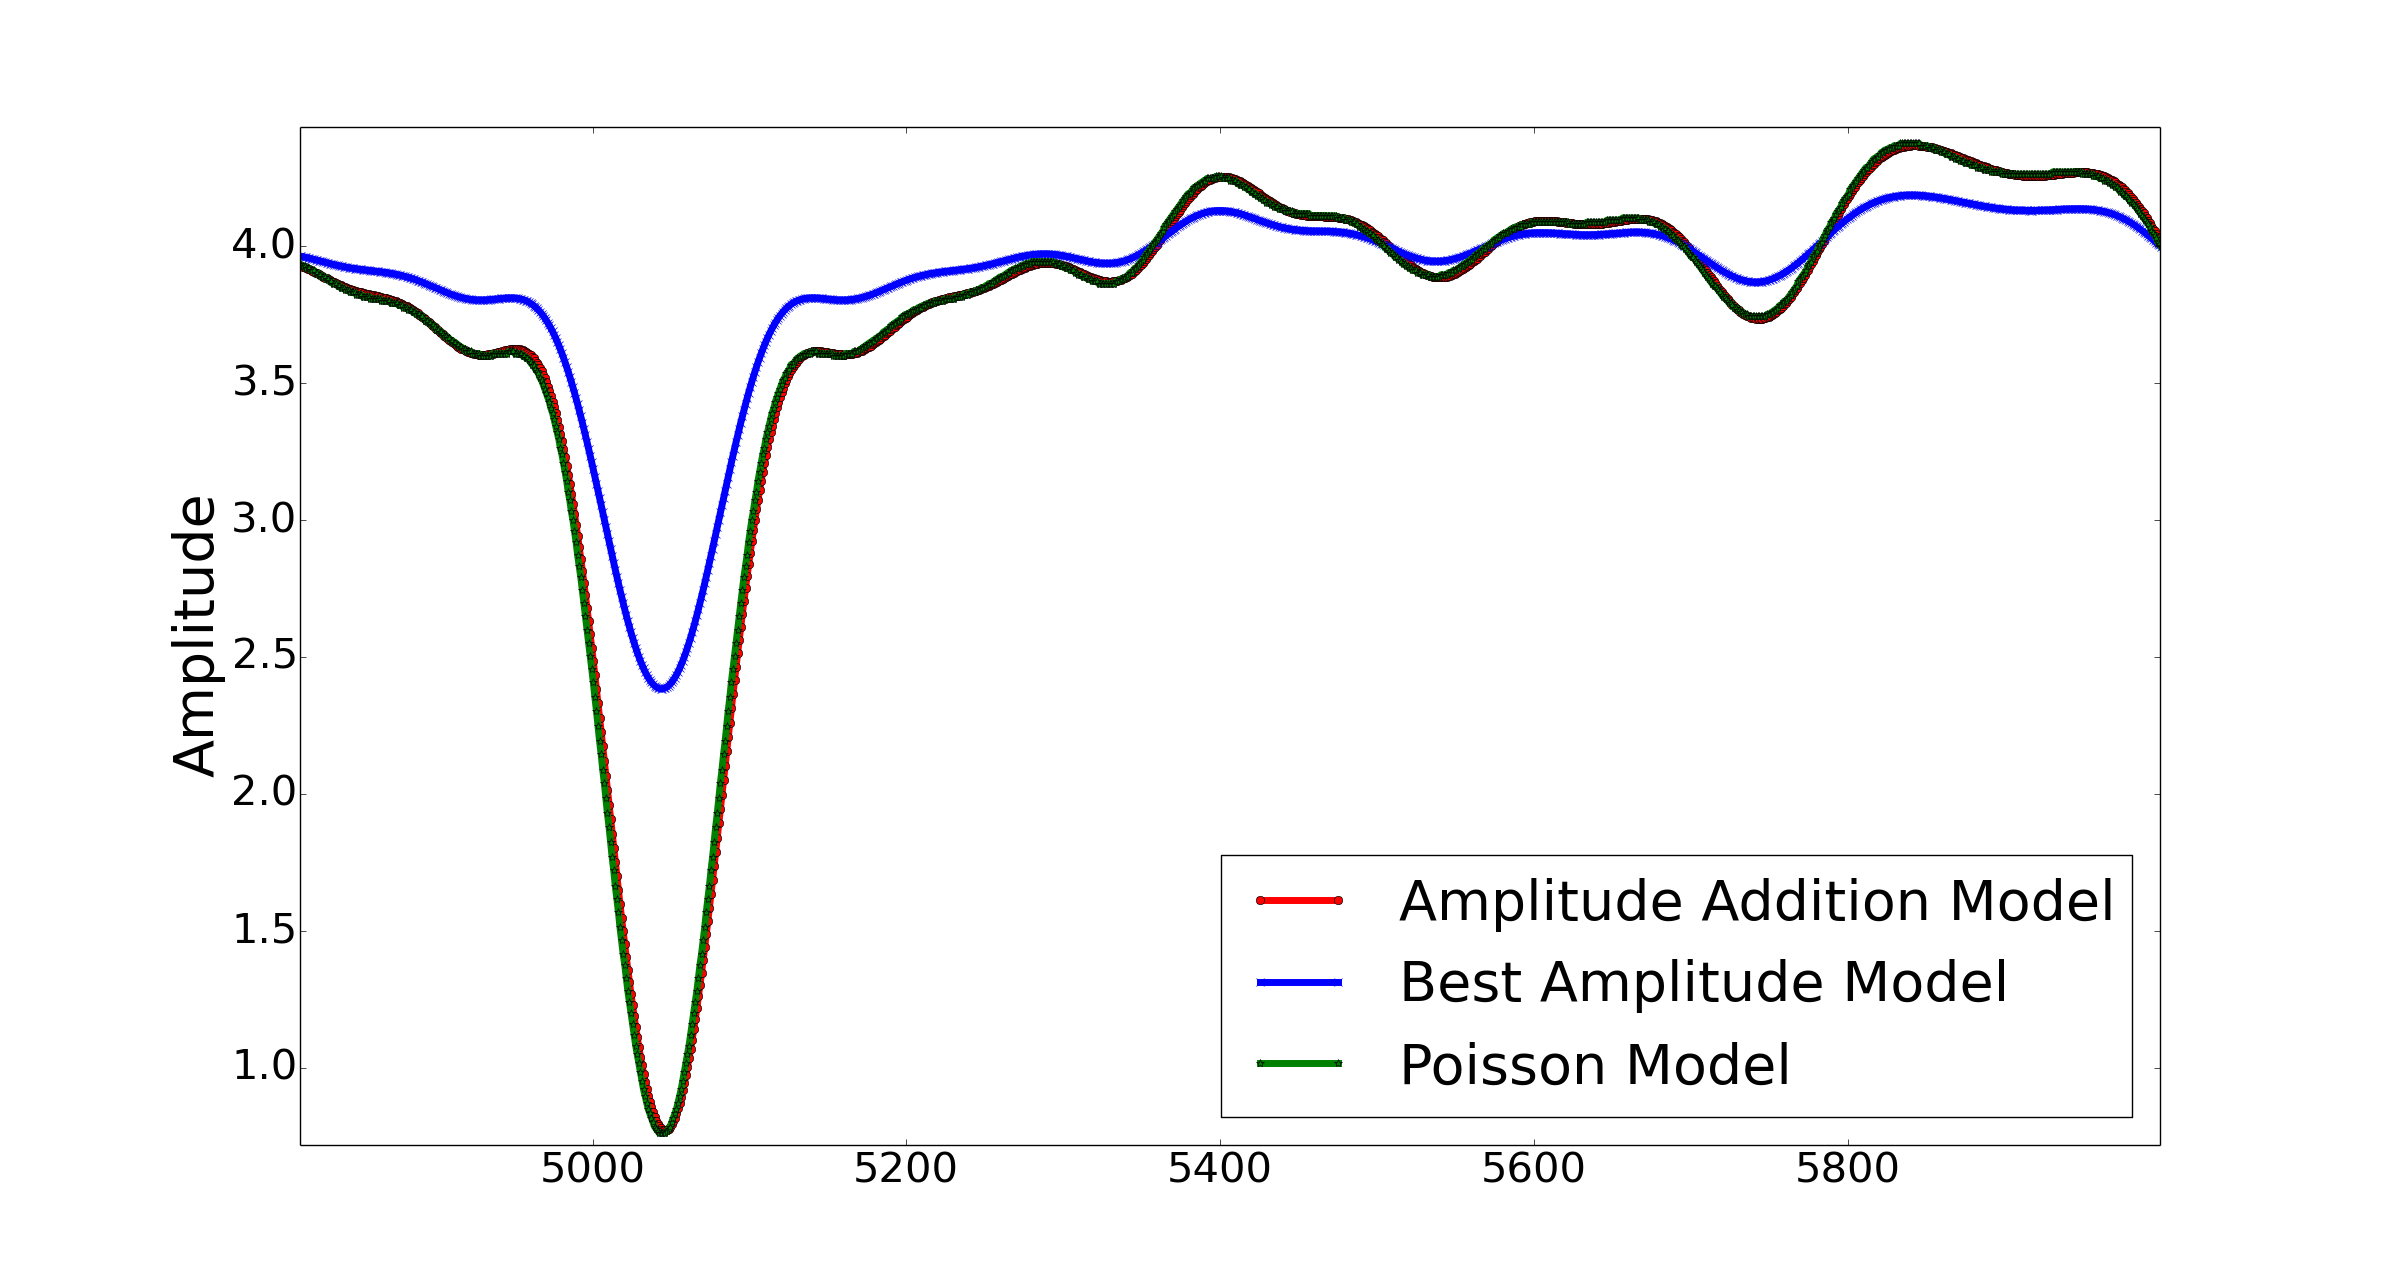
\includegraphics[width=0.7\linewidth]{Abbildungen/stand_der_technik/BAM_AAM}
	\caption{Vergleich $l$ Best Amplitude Model und $l$ Addition Amplitude Model Quelle \cite{Jovan.2016}}
	\label{fig.BAM_AAM_Vergleich}
\end{figure}

% sollte ich hier vllt auch die Tabelle von Seite 5 reinpacken, welche AAM und BAM vergleicht?
% hier noch von Marvin reinschreiben, wie er die alpha und beta Werte für die Gamma-Funktion berechnet, und rausarbeiten, dass ich nur sein Paper zitiere, weil er hier auf die Occupancy-Grids eingeht.
Eine genauere Beschreibung der Kalkulation des Formfaktors $\alpha$ und des inversen Skalenparameters $\beta$ der Gammafunktion findet sich in \cite{Stuede.2020}. Hier wird der Parameter $\lambda$ für jede Zelle eines 2D-Gitters berechnet. Die Wahrscheinlichkeit
für die Anzahl $N$ an Aktivitäten innerhalb eines Zeitintervalls in einer Zelle des Gitters kann dargestellt werden über:
\begin{equation}
	P_\ind{ij \tau} (N(t) = k) = \frac{(\lambda_\ind{ij \tau}(t-t_\tau))^k}{k!} e^\ind{-\lambda_\ind{ij\tau} (t- t_\tau)}
\end{equation}
wobei $\lambda_\ind{ij \tau}$ für die Rate an Aktivitäten der Zelle $(i,j)$ innerhalb des Zeitintervalls $\tau$ steht. Die der Zelle zugehörigen Parameter $\alpha_\ind{ij\tau}$ sowie $\beta_\ind{ij\tau}$ werden inkrementell für jeden Zeitschritt bestimmt $\sigma$  mittels der Vorschrift:
\begin{equation}
	\alpha_\sigma = \alpha_\ind{\sigma - 1} + x_\sigma \boldsymbol{l}_D (\boldsymbol{x}_R, t_\sigma),  \beta_\sigma = \beta_\ind{\sigma - 1} + \boldsymbol{l}_D (\boldsymbol{x}_R, t_\sigma )
\end{equation}
Als Anfangswerte werden $\alpha_0 = \beta_0 = 1 $ gewählt. Die Indikator-Funktion $\boldsymbol{l}_D (\boldsymbol{x}_r, t_\sigma)$ resultiert hierbei aus dem Detektionsbereich eines Roboters bei der Pose $\boldsymbol{x}_R$. Die a-posteriori erwarteten Werte der Aktivitätenrate $\lambda$ und ihrer Varianz berechnen sich nun für jedes Intervall zu:
\begin{equation}
	\hat{\lambda}_\ind{ij\tau} = E[\lambda_\ind{ij\tau}] = \frac{\alpha_\ind{ij\tau}}{\beta_\ind{ij}\tau},	Var[\lambda_\ind{ij\tau}] = \frac{\alpha_\ind{ij\tau}}{\beta_\ind{ij\tau}^2}
\end{equation}



		\chapter{Tipps zur Erstellung der Arbeit}
Im Folgenden sind einige Tipps zur schriftlichen Ausarbeitung zu finden, z.\,B. zur korrekten Darstellung von Gleichungen und Grafiken oder zum Bezug der dazu notwendigen Software. Grundsätzlich lassen sich unter folgendem Link Hilfestellungen zu den meisten Problemen bei der Erstellung Arbeit finden: http://bfy.tw/Bq9t

%%%%%%%%%%%%%%%%%%%%%%%%%%%%%%%%%%%%%%%%%%%%%%%%%%%%%%%%%%%%%%%%%%%%%%%%%%%%%%%%%%%%

\section{Darstellung von Gleichungen}
\label{sec.Gleichungen}
Der am imes verwendete Formelsatz entspricht der DIN 1338 und lässt sich auch in sämtlichen Skripten des imes wiederfinden, \zB in Robotik I, Robotik II oder Mechatronische Systeme.

Grundsätzlich gilt: Variablennamen werden kursiv gesetzt (auch wenn diese als Index benutzt werden, \zB $a_i$), beschreibende Indizes (z.\,B. $b_\ind{Reifen}$ oder $b_\ind{R}$) und allgemeine Funktionen (\zB Sinus- oder e-Funktion) aufrecht:

\begin{equation}
\label{eq:bsp_1}
	f(t) = \int\limits_{t_\ind{start}}^{t_\ind{end}} \sin(\omega t) \ind{d}t.
\end{equation}

Bei der ersten Verwendung von Variablen sollten diese unmittelbar vor oder nach der Gleichung im Text erläutert werden, in diesem Fall die exemplarische Funktion $f(t)$, Start- und Endzeitpunkt $t_\ind{start}$ bzw. $t_\ind{end}$, Kreisfrequenz $\omega$ und Zeit $t$. 


Matrizen und Vektoren werden fett gedruckt dargestellt. Matrizen werden mit großen, Vektoren mit kleinen Buchstaben bezeichnet. In der Gleichung

\begin{equation}
\label{eq:bsp_2}
	\boldsymbol{q} = (q_1, q_2, ..., q_n)^\mathrm{T}
\end{equation}

beschreibt $\boldsymbol{q}$ den Vektor mit allen Gelenkwinkeln, $q_1$ hingegen den Gelenkwinkel der ersten Achse. Zahlreiche weitere Beispiele zur Darstellung von Formeln können in den oben genannten Skripten nachgeschlagen werden.

Weitere Beispiele für korrekten Formelsatz:

\textbf{TODO -> versch. Stellen aus Skripten suchen und Code kopieren}

%%%%%%%%%%%%%%%%%%%%%%%%%%%%%%%%%%%%%%%%%%%%%%%%%%%%%%%%%%%%%%%%%%%%%%%%%%%%%%%%%%%%

\section{Darstellung von Grafiken}

Grafiken sollten nach Möglichkeit als Vektorgrafiken (z. B. .eps, .pdf) exportiert und in LaTeX eingebunden werden. Die Schriftart sollte der Schriftart der restlichen Arbeit entsprechen (Times). Die Schriftgröße in der Grafik sollte kleiner oder gleich der Größe des Fließtextes sein (nach eigenem Ermessen, solange die Lesbarkeit noch gegeben ist). Auch bei Abbildungen sind die Formatierungsschriften aus \Sec{Gleichungen} einzuhalten. Ein Beispielplot aus Matlab ist in \bild{Template} dargestellt. Das Skript zur Erstellung des Plots in Matlab ist unter template\_einfach.m zu finden.

\begin{figure}[!ht]
	\begin{center}
		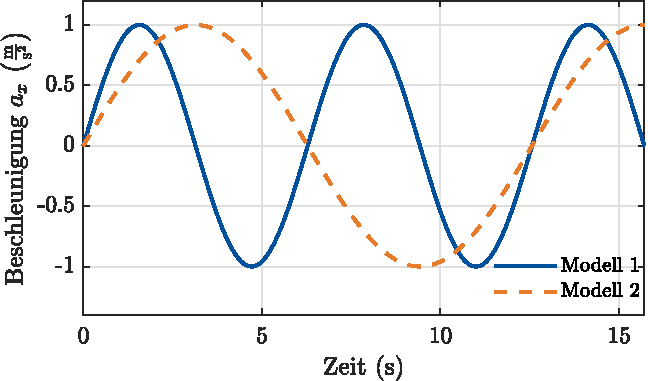
\includegraphics[]{template_einfach}
		\caption{Vergleich der zeitlichen Beschleunigungsverläufe der beiden Modellierungsansätze Hü (blau) und Hott (orange gestrichelt)}
		\label{fig.Template}
	\end{center}
\end{figure}

%%%%%%%%%%%%%%%%%%%%%%%%%%%%%%%%%%%%%%%%%%%%%%%%%%%%%%%%%%%%%%%%%%%%%%%%%%%%%%%%%%%%

\section{Software}
\subsection{Matlab, Corel}
Für Matlab und Corel sind an der Uni Hannover kostenlose Campuslizenzen verfügbar. Anleitungen zum Bezug sind unter https://www.luis.uni-hannover.de/softwarekatalog.html zu finden. Für Corel existiert am imes ein Plugin zur Nutzung von LaTeX-Befehlen. Das Plugin und die zugehörige Anleitung sind im Vorlagenordner zu finden. Alternativ zu Corel kann auch die freie Software Inkscape genutzt werden (https://inkscape.org).

\subsection{LaTeX}
Vorschläge für TeX-Distributionen:
\begin{itemize}
	\item MiKTeX (Windows): https://miktex.org/
	\item TeXLive (allg.): http://www.tug.org/texlive/
\end{itemize}

Vorschläge für Texteditoren:
\begin{itemize}
	\item TeXnicCenter (Windows): http://www.texniccenter.org/
	\item TeXMaker (allg.): http://www.xm1math.net/texmaker/
\end{itemize}

%%%%%%%%%%%%%%%%%%%%%%%%%%%%%%%%%%%%%%%%%%%%%%%%%%%%%%%%%%%%%%%%%%%%%%%%%%%%%%%%%%%%

\section{Literaturverweise}
Beispiele für Literaturverweise sind im Literaturverzeichnis zu finden, z.\,B. Journalbeitrag \cite{Ber59}, Konferenzbeitrag \cite{Hussong08}, Buch \cite{Wintermantel09}. Sofern nicht explizit anders eingestellt, taucht nur diejenige Literatur im Verzeichnis auf, auf die in der Arbeit verwiesen wird.

%%%%%%%%%%%%%%%%%%%%%%%%%%%%%%%%%%%%%%%%%%%%%%%%%%%%%%%%%%%%%%%%%%%%%%%%%%%%%%%%%%%%

\section{Eigene Befehle in LaTeX}
In LateX können auch eigene Befehle definiert und genutzt werden, \zB zur Verwendung immer wiederkehrender Formelzeichen. So kann beispielsweise ein Koordinatensystem $\ks{A}$ direkt mit dem Befehl \textbackslash ks\{A\} eingefügt werden. Eine Liste der Befehle ist in der Datei befehle.sty zu finden.


		\chapter{Betreuer- und/oder projektspezifische Anmerkungen}
Für Ergänzungen zur Vorlage, die nicht allgemeingültig sind, bitte ausschließlich dieses Kapitel nutzen!

ToDos für die Vorlage:
\begin{itemize}
	\item Aufgabenstellung direkt ins Dokument, Platzhalter-pdf, manuell reinsortieren?
	\item mehr Beispiele für Formelsatz aus versch. Skripten reinkopieren
	\item Befehle.sty erläutern
\end{itemize}
		\chapter{(Beispielkapitel) Robotersysteme}

Das folgende Kapitel soll als Beispielkapitel dienen. Nach der Kapitelüberschrift wird der Kapitelinhalt in ein paar Sätzen beschrieben.
Hier steht weiterer Text.

\section{PR2}

Der PR2 (Willow Garage Inc., Menlo Park, USA) ist ein \textbf{\textit{menschenähnlicher}} Serviceroboter, der seinen Dienst in Wohnräumen verrichten soll und derzeit im sogenannten PR2 Beta-Programm von elf Forschungseinrichtungen über einen Zeitraum von zwei Jahren getestet wird \cite{WillowGarage2010}.
Hier steht weiterer Text.  d

\begin{figure}[!ht]
	\centering
	\subfigure[]{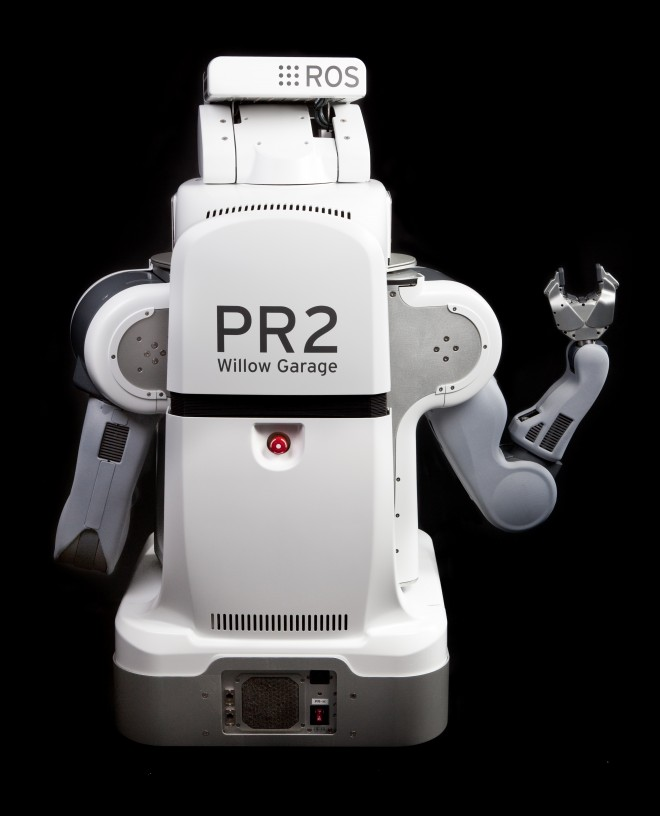
\includegraphics[height=50mm]{PR2-1}}
	\hspace{5mm}
	\subfigure[]{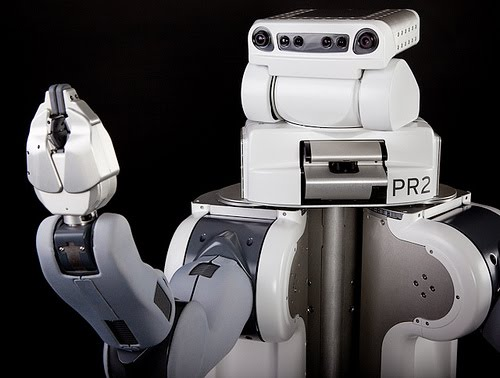
\includegraphics[height=50mm]{PR2-2}}
	\hspace{5mm}
	\subfigure[]{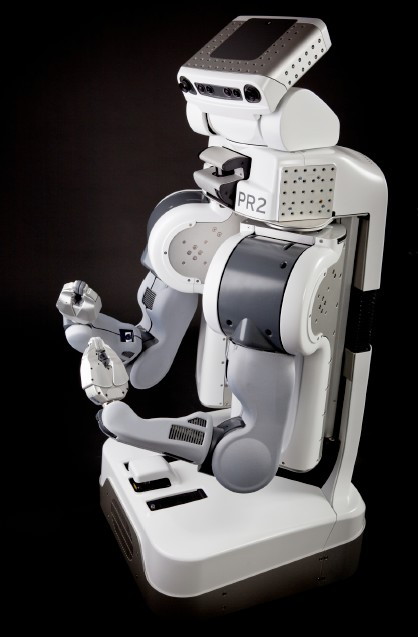
\includegraphics[height=50mm]{PR2-3}}
	\caption{Serviceroboter PR2 von Willow Garage (Quelle: Willow Garage))}
	\label{fig.PR2}
\end{figure}

Ausgestattet ist der PR2 mit zwei Armen, die jeweils sieben Freiheitsgrade haben und an deren Enden ein Greifer montiert ist, siehe \bild{PR2}. Die Sensorik des Armes besteht aus einer Kamera am Unterarm und Druck- sowie Beschleunigungssensoren am Greifer. Die Nutzlast eines Arms ist mit \SI{1,8}{kg} ausgewiesen. Weiterhin verfügt der Roboter über einen dreh- und schwenkbaren Kopf, in dem eine 5-Megapixel Farbkamera, ein LED-Texturprojektor und zwei Stereokameras integriert sind, wobei eine Kamera für die Fernsicht und die andere für die Objektmanipulation genutzt wird. Unterhalb des Kopfes ist ein schwenkbarer Laserscanner und ein Inertialsensor verbaut. Die Position des Oberkörpers lässt sich in der Höhe zwischen \SI{1330}{mm} und \SI{1645}{mm} (Gesamthöhe) variieren. Angetrieben wird die omnidirektionale Basis von vier gelenkten Rädern, die eine maximale Geschwindigkeit von \SI{3,6}{\kilo\metre\per\hour} ermöglichen. Die quadratische Basis hat eine Kantenlänge von \SI{668}{mm}. Als Recheneinheit stehen zwei Server zur Verfügung, die jeweils auf acht CPU-Kernen rechnen und dabei auf 24\,GB Arbeitsspeicher zugreifen können. Als Betriebssystem wird Ubuntu verwendet, auf dem das Robot Operating System, kurz ROS, die Grundlage für die Datenverarbeitung bildet. Da ROS innerhalb dieser Arbeit ebenfalls zum Einsatz kommt, wird dieses in \Sec{ROS} vorgestellt und an den entsprechenden Stellen weiter erläutert. Die Kosten für einen PR2-Roboter belaufen sich derzeit auf etwa \SI{400 000}{\text{US-Dollar}}\footnotemark. Mit Hilfe des PR2 wurden von den zuvor erwähnten Beta-Testern Szenarien bewältigt, die innerhalb des menschlichen Wohnraumes auftreten können. An der TU München hat ein PR2-Roboter beispielsweise zusammen mit einem anderen Robotersystem einen Pfannkuchen gebacken \cite{TUM2011}.
\footnotetext{Der angegebene Preis wurde am 16.08.2011 der Website http://www.willowgarage.com/pages/pr2/order entnommen und versteht sich exklusive Steuern und Versandkosten.}

\section{ROS}
\label{sec.ROS}

Hier steht weiterer Text.

\begin{table}
	\centering
	\caption{Technische Daten der youBot Plattform}\label{tab.TechSpecYouBotBase}
	\vspace*{-3mm}
	\begin{tabular}{lcr}
        \toprule
		Bezeichnung		& Formelzeichen	&              \\
		\midrule
		Gesamtlänge 	& $a$           & \SI{530}{mm} \\
		\rowcolor{Snow2}
		Gesamtbreite 	& $b$           & \SI{350}{mm} \\
		Höhe			& $h$           & \SI{106}{mm} \\
		Radstand		& $l$           & \SI{470}{mm} \\
		\bottomrule
	\end{tabular} 
\end{table}

\begin{lstlisting}[label=source.launchHokuyo,caption=Launchfile zum Start der hokuyo\_node]
<!-- launch hokuyo node -->
<node pkg="hokuyo_node" type="hokuyo_node" name="hokuyo_node" output="screen">
	<param name="port" value="/dev/ttyACM0"/>
	<param name="frame_id" value="/base_laser_front_link"/>
</node>
\end{lstlisting}
    %\nocite{*}                             % alle Literaturquellen einbinden, sonst werden nur die zitierten
                                            % Quellen im Literaturverzeichnis angezeigt (ist Geschmackssache).
                                            % eher nicht verwenden, außer man hat einen guten Grund
    \appendix                               % Anhang starten, jedes weitere Kapitel bekommt jetzt einen Buchstaben
    \chapter*{Anhang}                       % Anhang als Chapter
    \addcontentsline{toc}{chapter}{Anhang}
    %\thispagestyle{empty}                   % keine Kopfzeile, Seitenzahl u.a., leere Seite mit Überschrift Anhang
    %\setcounter{chapter}{1}                 % Chapter Counter auf 1 = im Anhang A
    %\setcounter{equation}{0}                % Equation Counter nullen
    %\newpage                                
    %\ihead{\normalfont Anhang}              % Kopfzeile auf Anhang setzen



    %% --- Ab hier der Anhang einfügen

    %\include{anhang_wheatstone}            % Anhang
    %\include{anhang_fehlerfortpflanzung}
		%\include{anhang_mgcEinstellungen}
		%\include{anhang_trafos}
		%\include{anhang_befestigen}
		%\include{anhang_datenblaetter}
    %% --- Anhang zu Ende
		
    \ihead{\normalfont\headmark}            % kolumnentitel innen
 
    %% --- Literaturverzeichnis
    {\sloppy \printbibliography}

\end{spacing}
\end{document}                              % fertig!

